% !TeX root = ../main.tex
% -*- coding: utf-8 -*-

\chapter{基于近边界数据的模型所有权推断方法分析}\label{5}

我们在开源数据集CIFAR-10\cite{krizhevsky2009learning},Heritage\cite{Heritage},Intel\_image\cite{Intel_image}上面进行实验,并选择ResNet18作为评估的源模型,VGG11作为对照的无关模型。本文使用的模型均在开源的预训练模型上进行训练。

\noindent\textbf{被盗模型:}我们设置了常见的几种模型盗窃方法,包括模型微调,模型剪枝(不同的剪枝率)和模型蒸馏,并在源模型的基础上得到被盗模型。

\section{实验设置}\label{5.1}

本文实验利用CIFAR-10,Heritage和Intel\_image三种数据集训练ResNet18,训练过程中Adam优化器并将学习率(Learning rate),迭代轮次(Epoch)和每批次大小(Batch size)分别设置为0.0001,200和64。蒸馏模型实验选择从Resnet18蒸馏至VGG11,蒸馏时将蒸馏温度设置为20并且教师模型比例$\alpha$=0.7,训练轮次是20。初始近边界数据生成采用$CW$-$L_2$算法,实验中选择有目标的生成方式,且学习率,迭代次数和二分搜索次数分别设置为0.001,1000和6,其他参数为默认值。私有近边界数据生成器采用DCGAN的基础结构,训练过程使用Adam优化器且将学习率,训练轮次和每批次大小分别设置为0.0002,8000和64。注意本发明最后微调源模型阶段需要交替使用源模型损失函数和微调目标边界的损失函数来微调源模型,具体设置为10个轮次交替一次且交替次数最多为10次。



\section{生成初始近边界数据的算法选择}\label{5.2}

本小节将对\ref{3}\ref{3.2}中提出的FGSM,IGSM,RFGSM和CW-$L_2$进行测试,我们均使用原作者发布的实现。FGSM,IGSM,RFGSM中均有一个用于界定噪声$\epsilon$的参数,且IGSM和RFGSM还包含一个重要的参数$\alpha$ 用来表示迭代次数。我们进行大量的实验探索选择合适的参数用于与CW-$L_2$进行比较。此外,CW-$L_2$的实验设置如\ref{5.1}所示。如表\ref{table:1}所示,CW-$L_2$生成的对抗性样例与目标分类边界的平均距离远比其他算法小。因此,本文使用该算法作为初始近边界数据生成算法。

\begin{table}[H]
	\centering
	\setlength{\arrayrulewidth}{0.5mm}
	\renewcommand\arraystretch{1.5}
	\caption{不同对抗性样本生成算法生成的数据与目标分类边界的平均距离}
	\label{table:1}
	\begin{tabular*}{13cm}{@{\extracolsep{\fill}} l c c c c}
		
		\hline
		数据集                    &   FGSM   &   IGSM   &  RFGSM  &   CW-$L_2$    \\
		\hline
\multirow{3}{6em}{CIFAR-10}      &    0.557  &   0.430  &  0.418   &    0.066     \\
		                         &    0.461  &   0.419  &  0.373   &    0.103     \\
		                         &    0.586  &   0.369  &  0.356   &    0.112     \\
		\hline
\multirow{3}{6em}{Heritage}      &    0.347  &   0.356  &  0.314   &    0.014     \\
		                         &    0.277  &   0.340  &  0.281   &    0.016     \\
		                         &    0.348  &   0.332  &  0.276   &    0.010     \\
		\hline
\multirow{3}{6em}{Intel\_image}  &    0.522  &   0.447  &  0.353   &    0.088     \\
		                         &    0.475  &   0.506  &  0.387   &    0.122     \\
		                         &    0.468  &   0.402  &  0.428   &    0.127     \\
		\hline		
	\end{tabular*}
\end{table}


\section{数据近边界特性的评估}\label{5.3}

如图\ref{CIFAR-10上不同分类边界下的近边界数据表现}图\ref{Heritage上不同分类边界下的近边界数据表现}图\ref{Intel-image上不同分类边界下的近边界数据表现}所示, 本文提出的近边界数据在所有盗窃模型中都表现出了靠近分类边界的特性。例如,我们的方法在全部数据集中,近边界数据在无关模型上表现出和目标分类边界没有关系。然而,在基于源模型的各种盗窃模型上近边界数据表现良好,尤其是模型修改方法破坏性较强如模型蒸馏时依旧表现出靠近目标分类边界的特性。注意我们此处使用的近边界数据的大小为64,换句话说,我们的方法在较小规模的近边界数据上依旧效果显著,可以想到的是当数据量增大时,我们的方法效果会更加明显。


\begin{figure}[htbp]%%图,[htbp]是浮动格式
	\centering
	\begin{minipage}[htbp]{0.49\linewidth}        %图片占用一行宽度的50%
		\hspace{2mm}
		\centering
		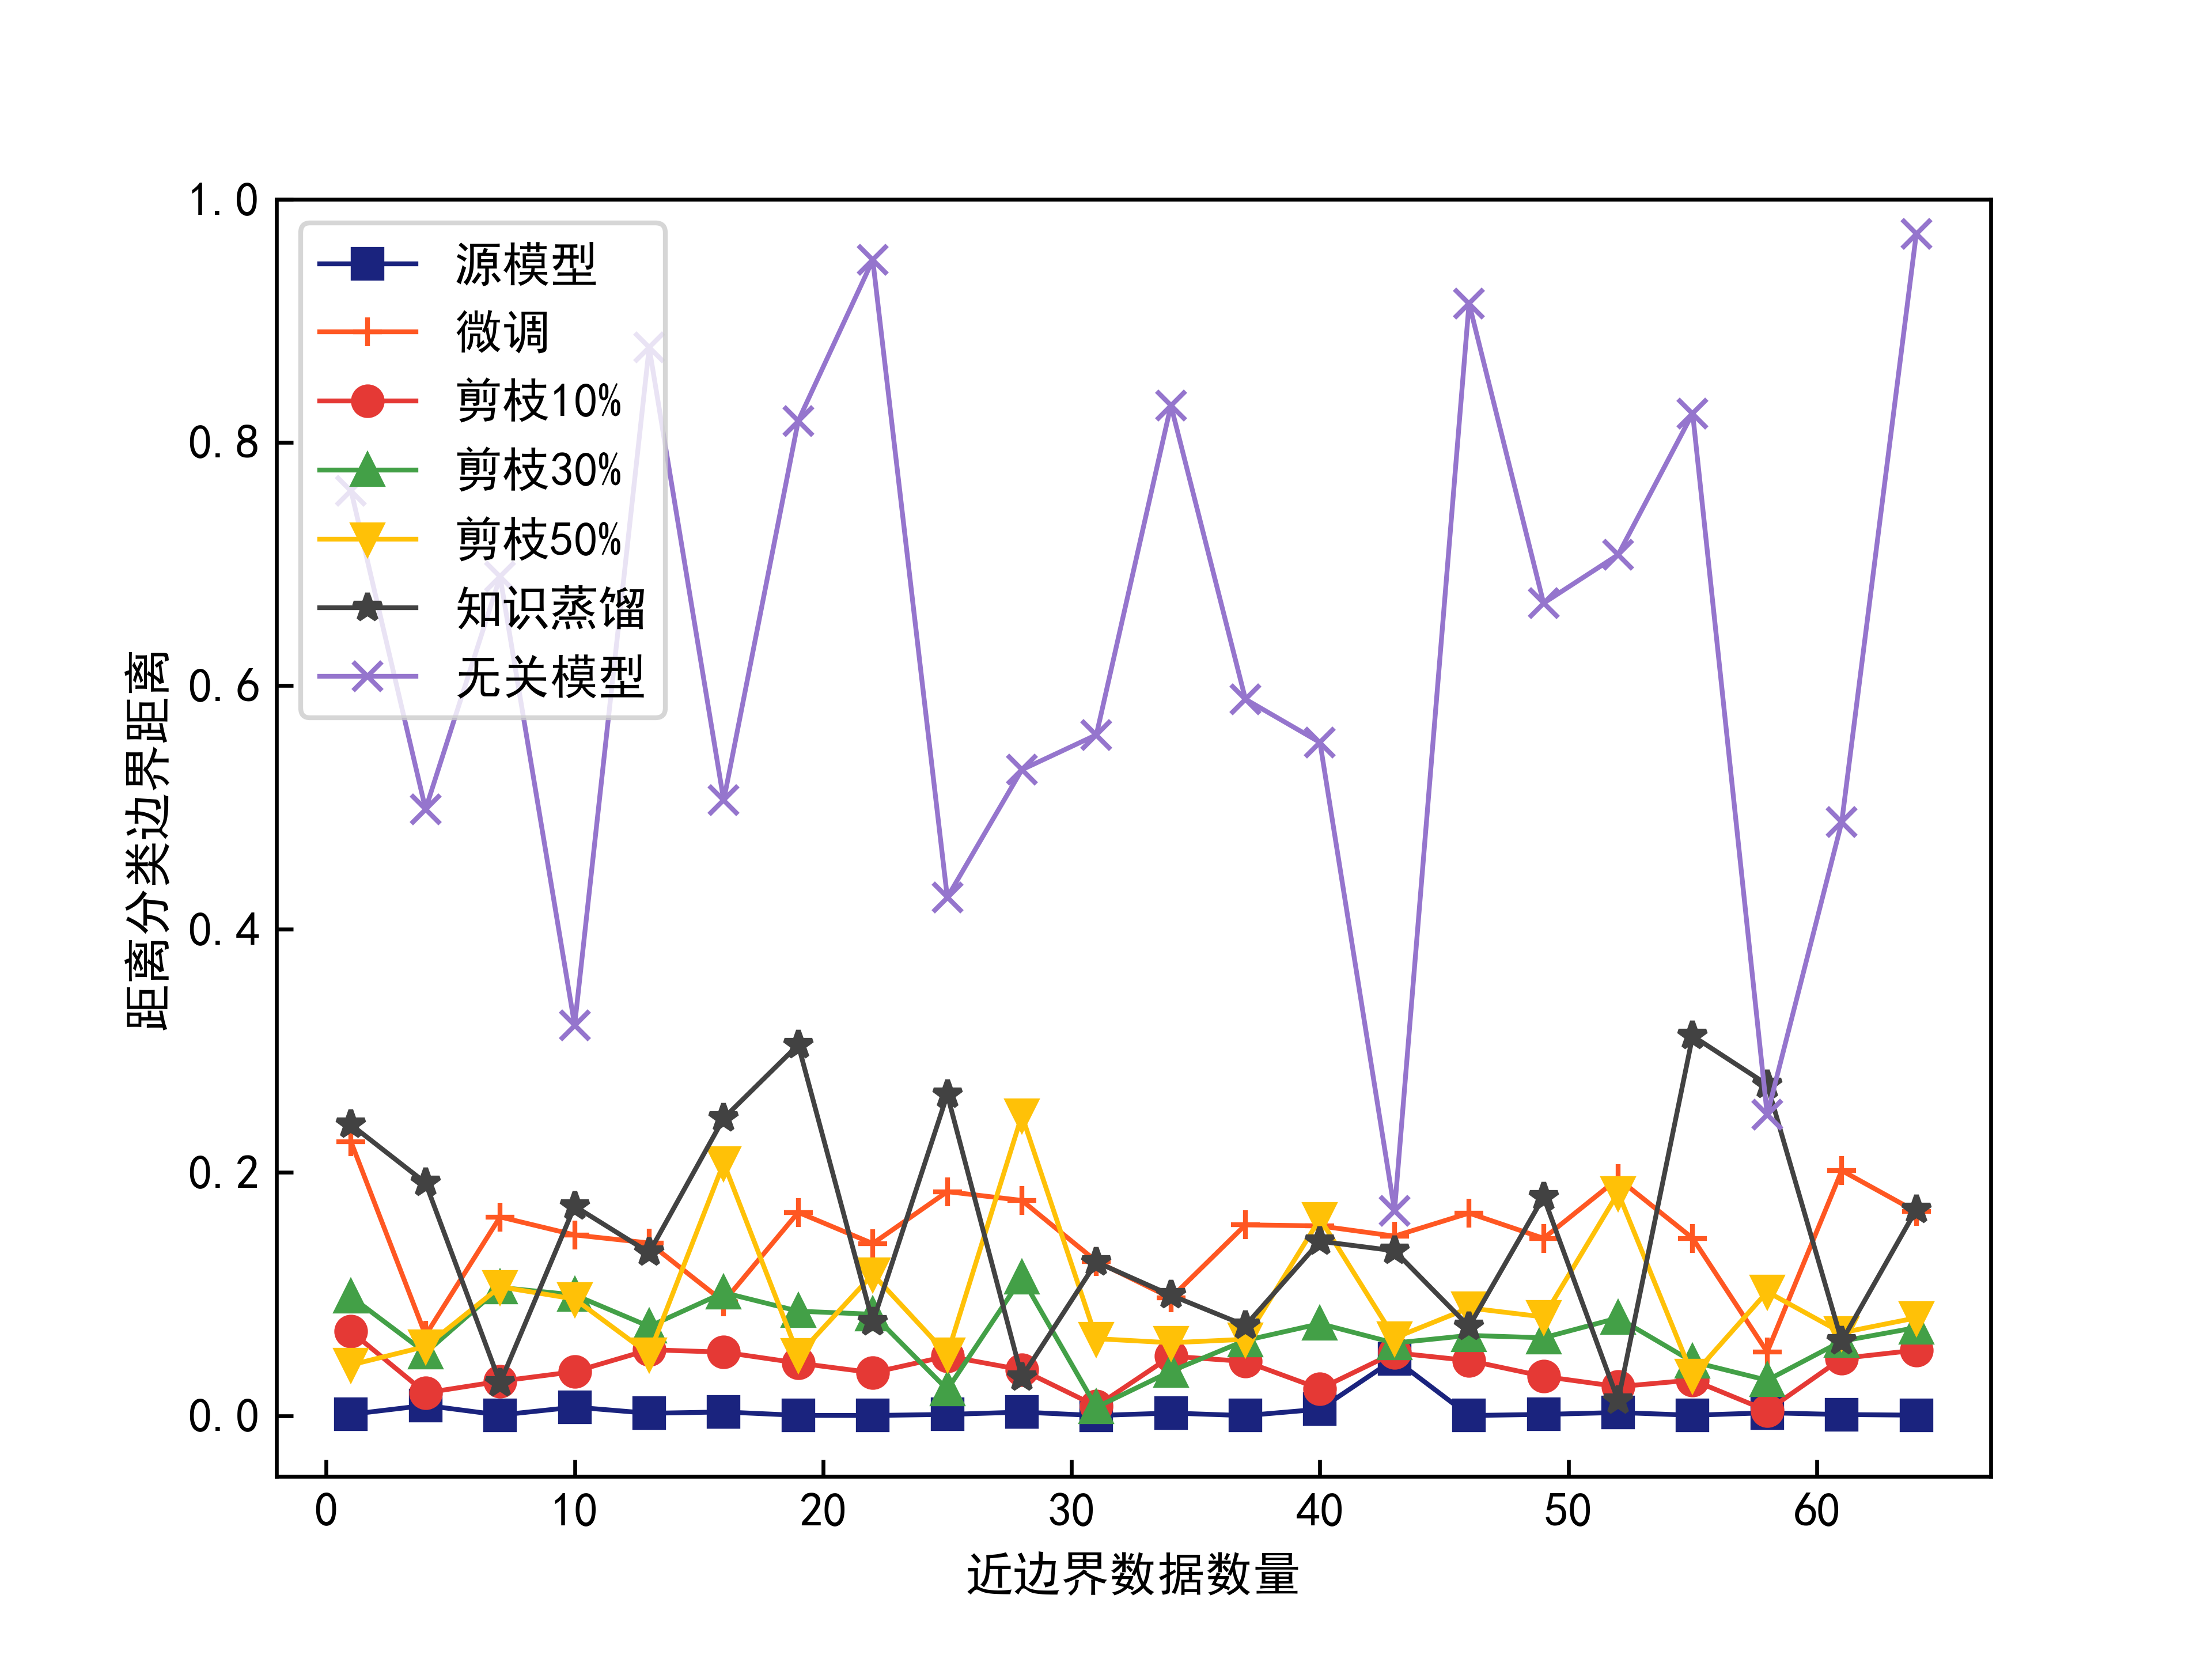
\includegraphics[width=7cm,height=4cm]{CIFAR-10-4-2-distance.png}
		\centerline{(a)分类边界1}
	\end{minipage}
	\begin{minipage}[htbp]{0.49\linewidth}        %图片占用一行宽度的50%
		\hspace{2mm}
		\centering
		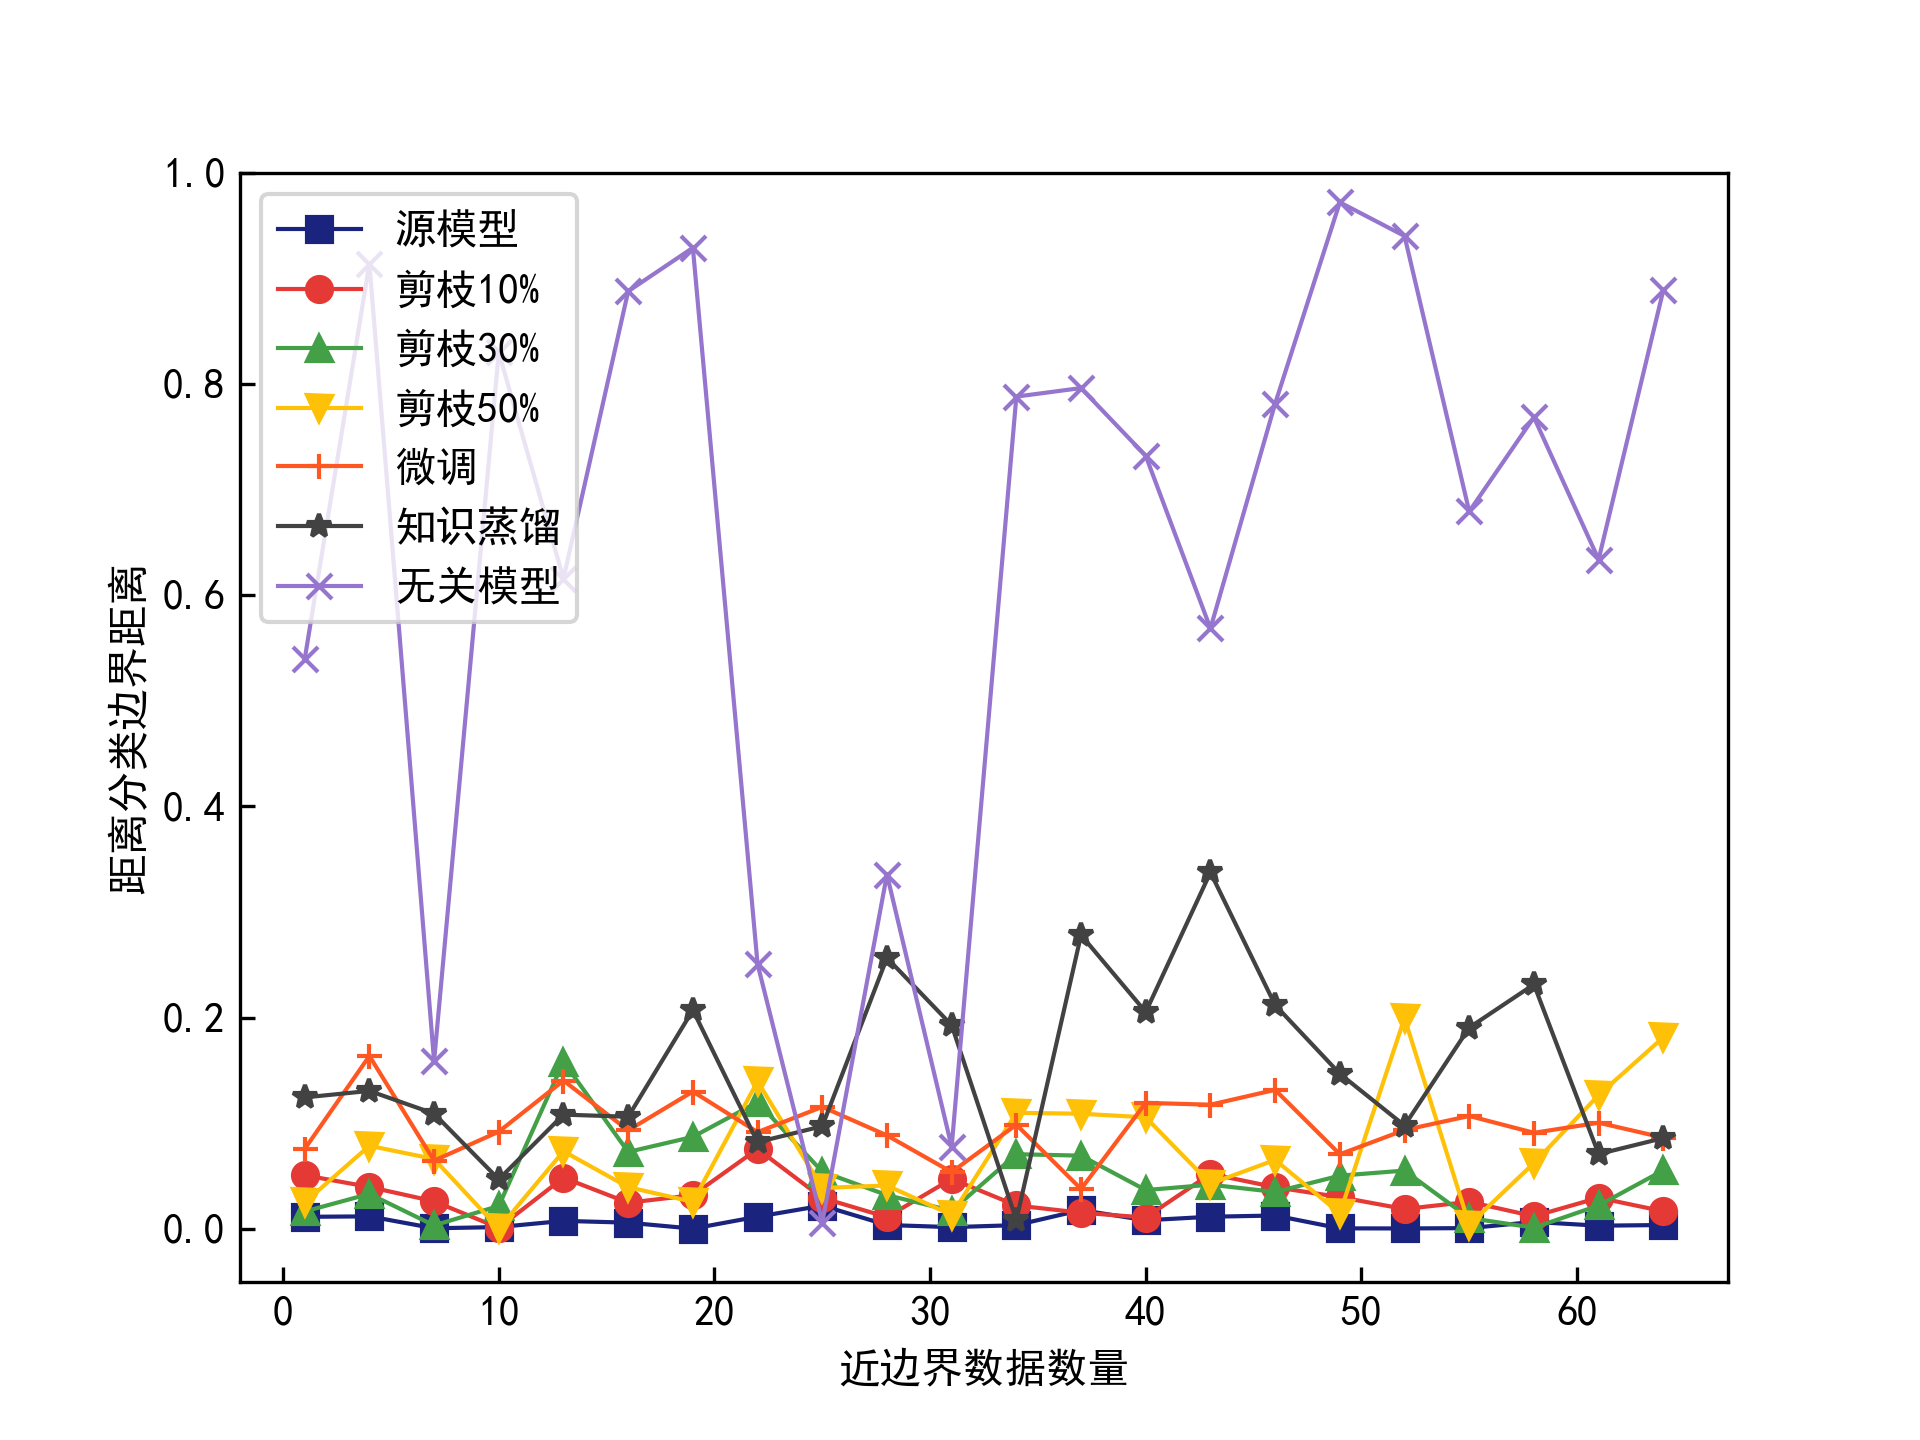
\includegraphics[width=7cm,height=4cm]{CIFAR-10-4-3-distance.png}
		\centerline{(b)分类边界2}
	\end{minipage}
	\begin{minipage}[htbp]{0.49\linewidth}        %图片占用一行宽度的50%
		\hspace{2mm}
		\centering
		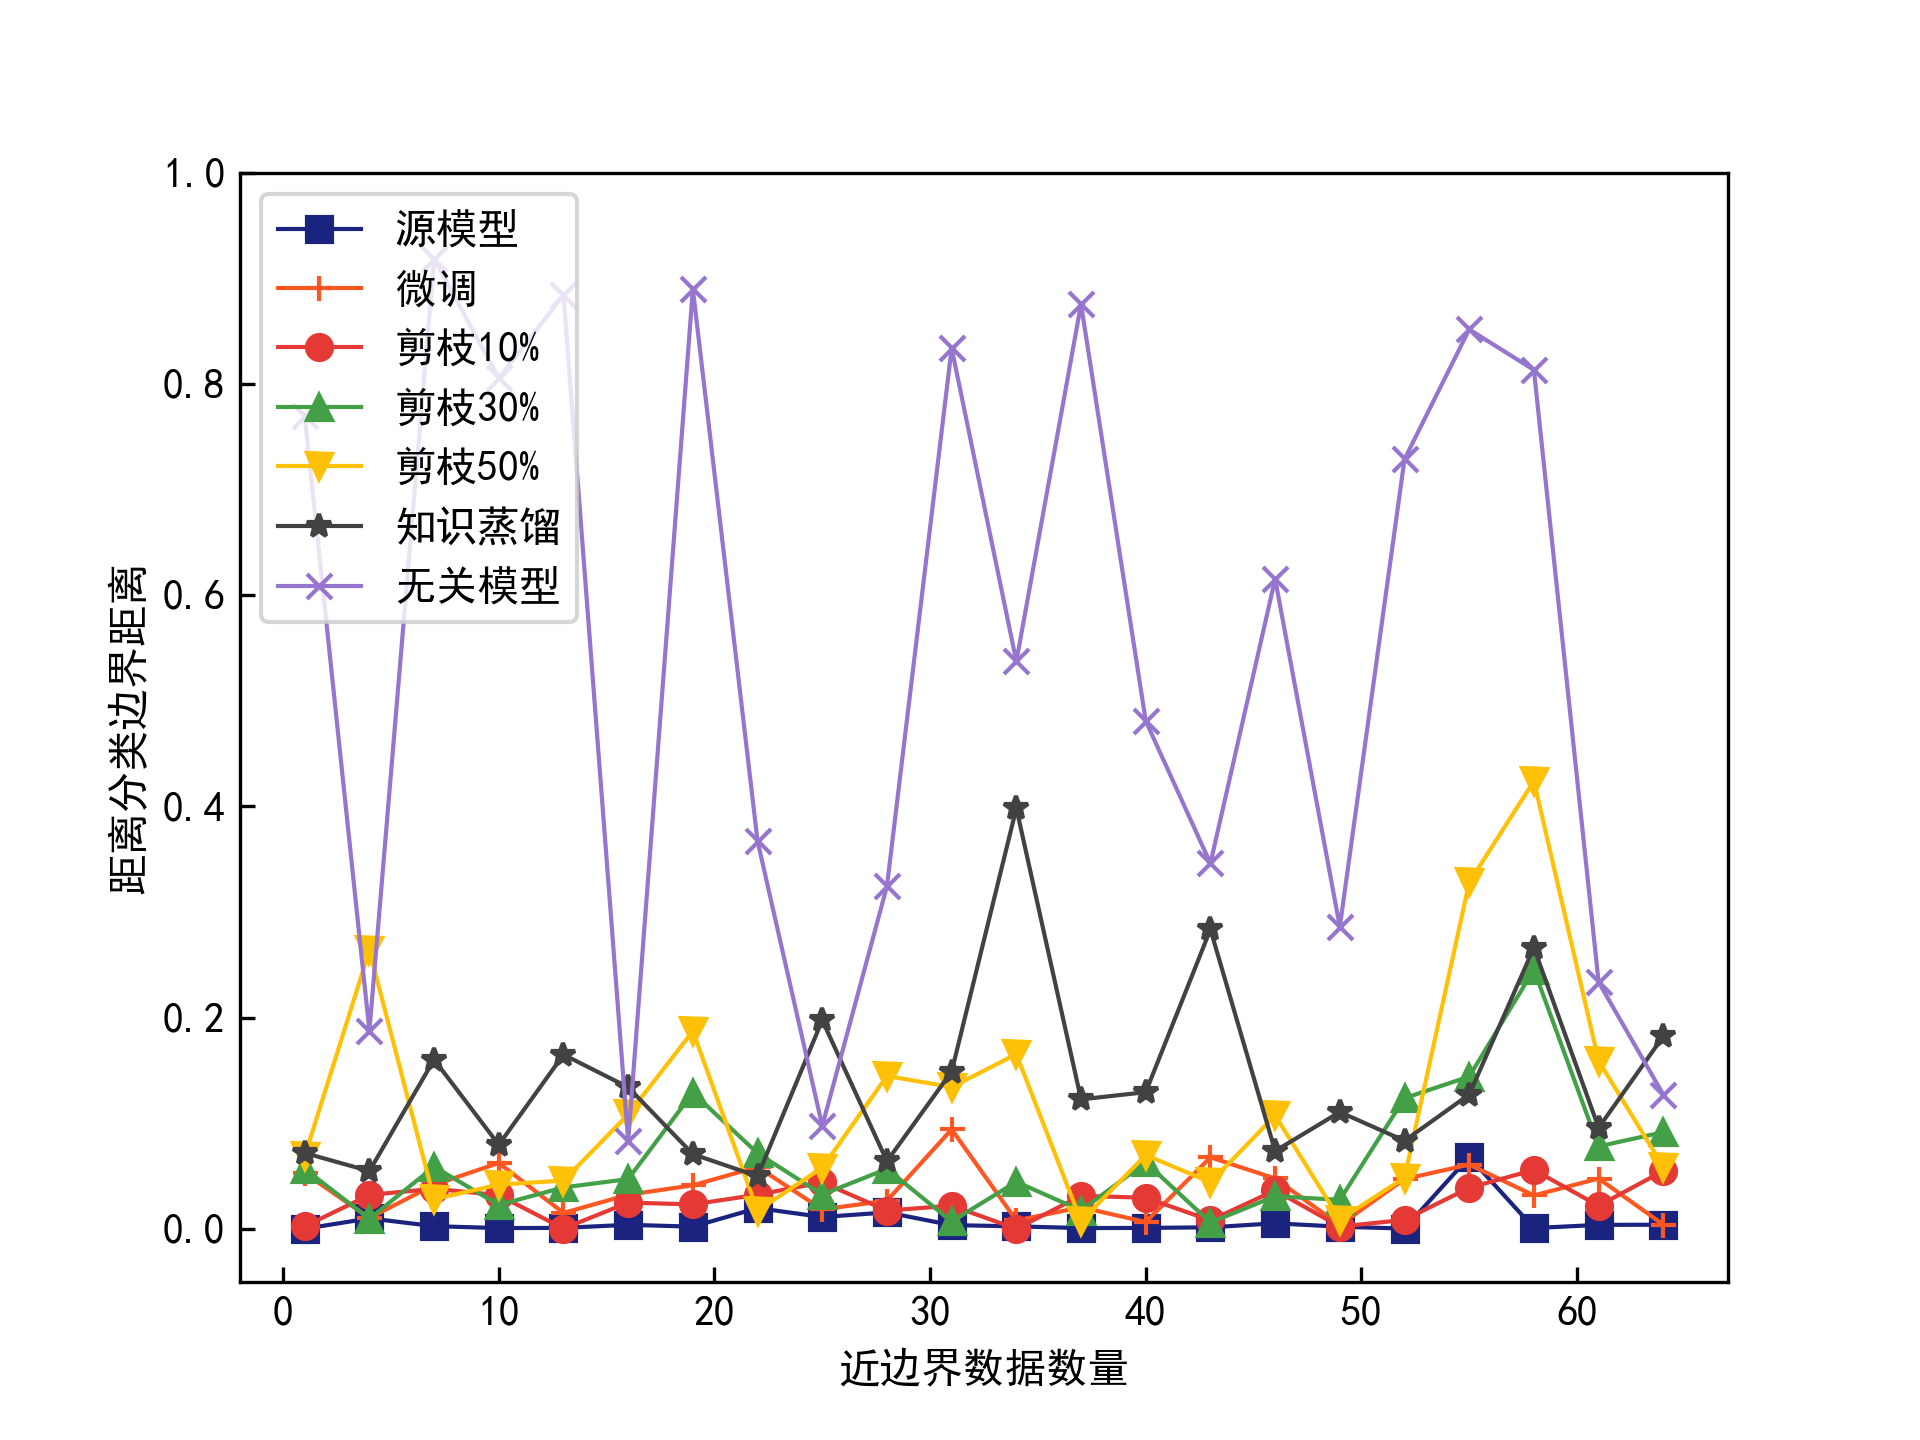
\includegraphics[width=7cm,height=4cm]{CIFAR-10-4-7-distance.png}
		\centerline{(c)分类边界3}
	\end{minipage}
	\begin{minipage}[htbp]{0.49\linewidth}        %图片占用一行宽度的50%
		\hspace{2mm}
		\centering
		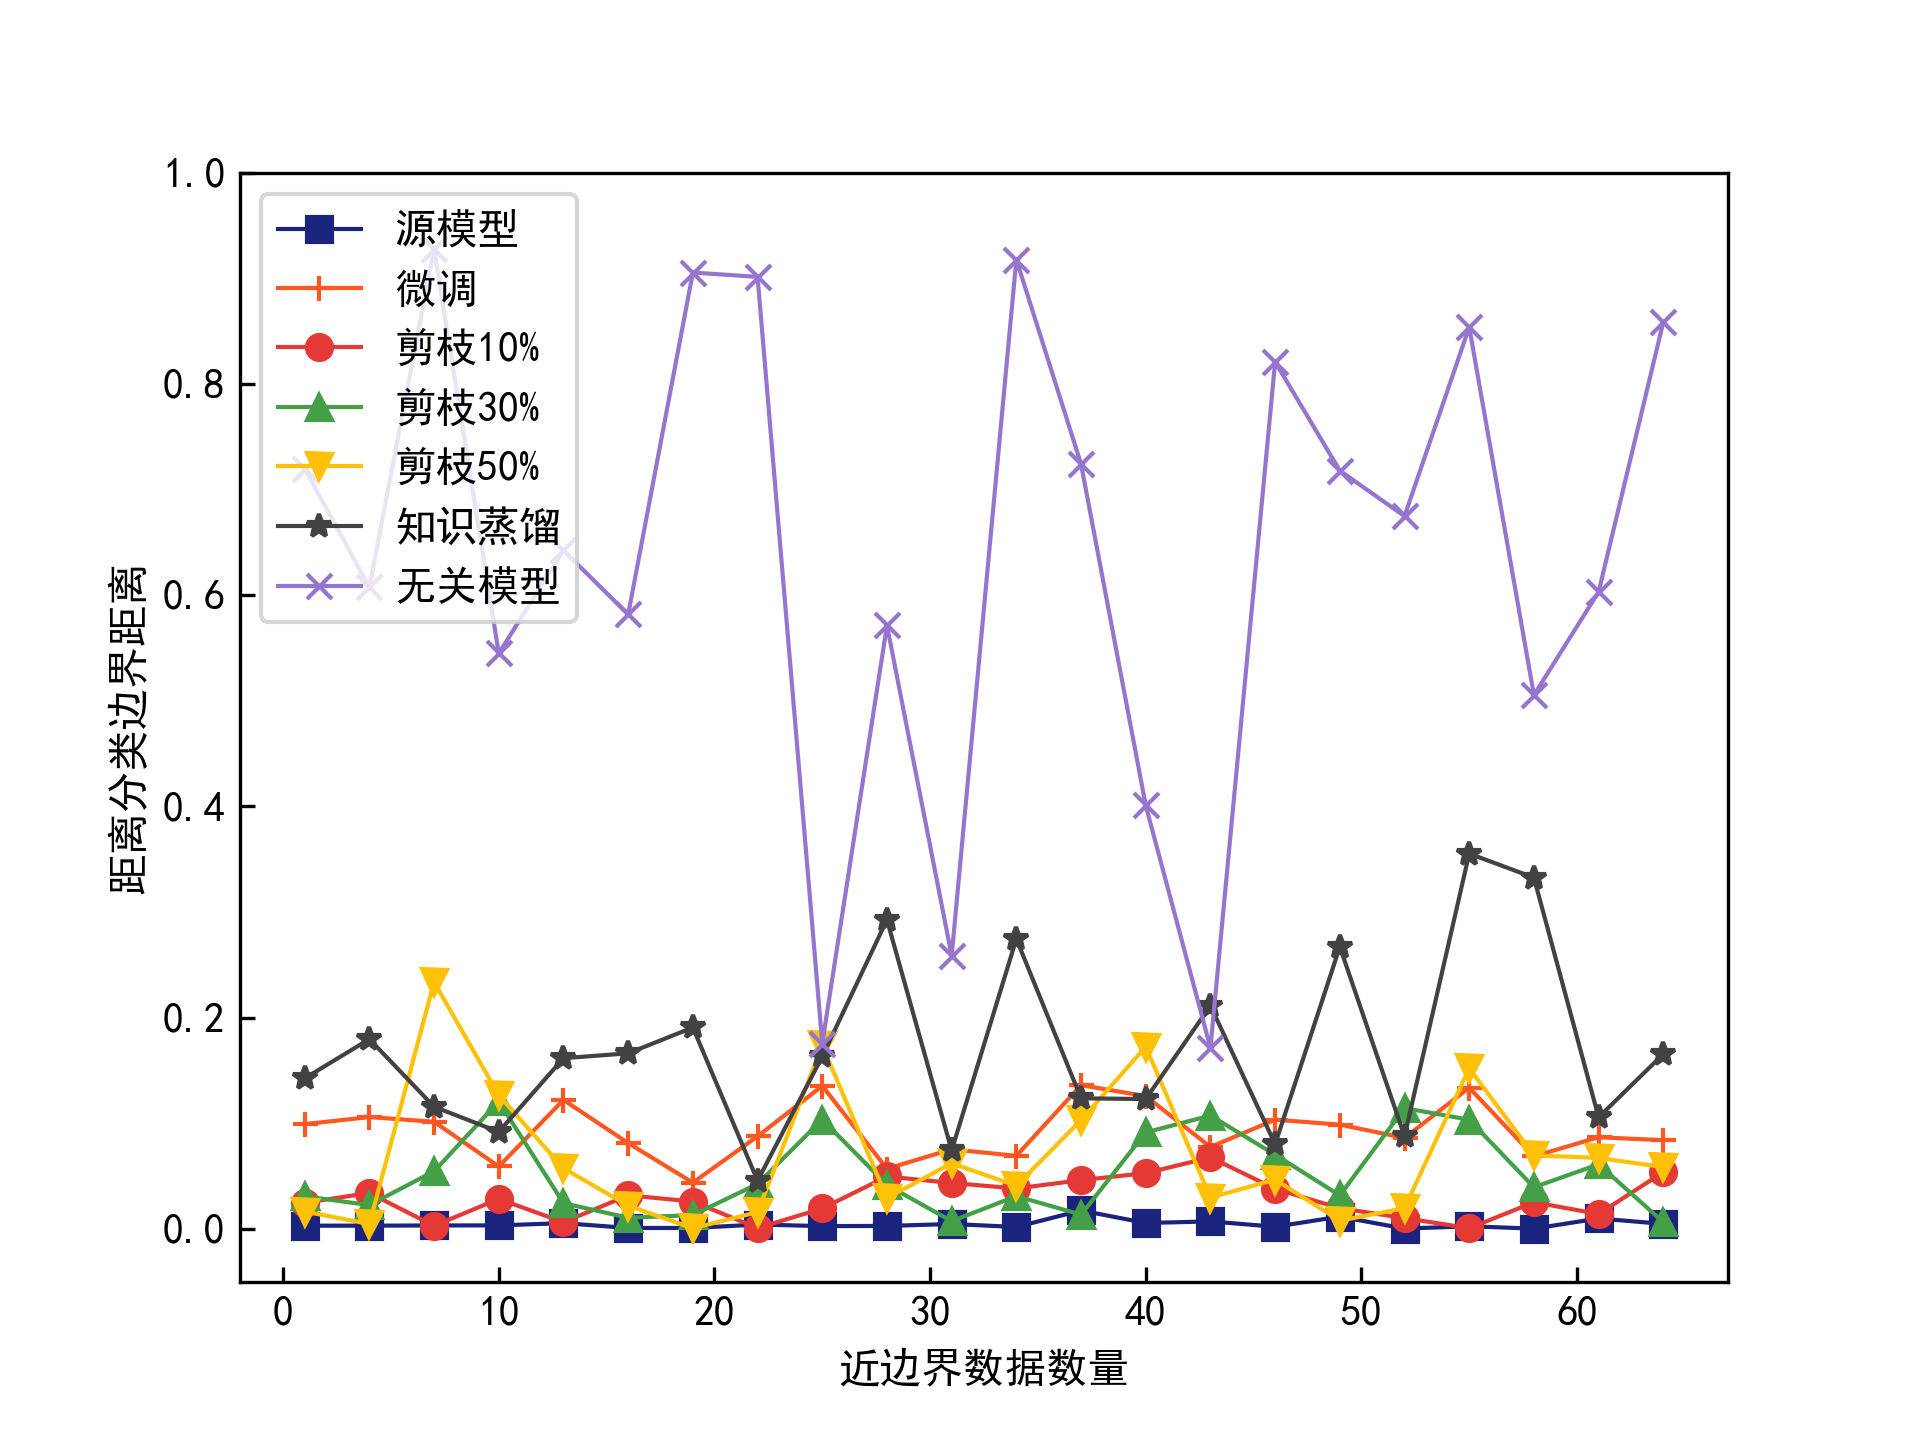
\includegraphics[width=7cm,height=4cm]{CIFAR-10-5-6-distance.png}
		\centerline{(d)分类边界4}
	\end{minipage}
\setlength{\abovecaptionskip}{7mm} %图片标题与图片距离
\caption{CIFAR-10上不同分类边界下的近边界数据表现}
\label{CIFAR-10上不同分类边界下的近边界数据表现}
\end {figure}

\begin{figure}[htbp]%%图,[htbp]是浮动格式
	\centering
	\begin{minipage}[htbp]{0.49\linewidth}        %图片占用一行宽度的50%
		\hspace{2mm}
		\centering
		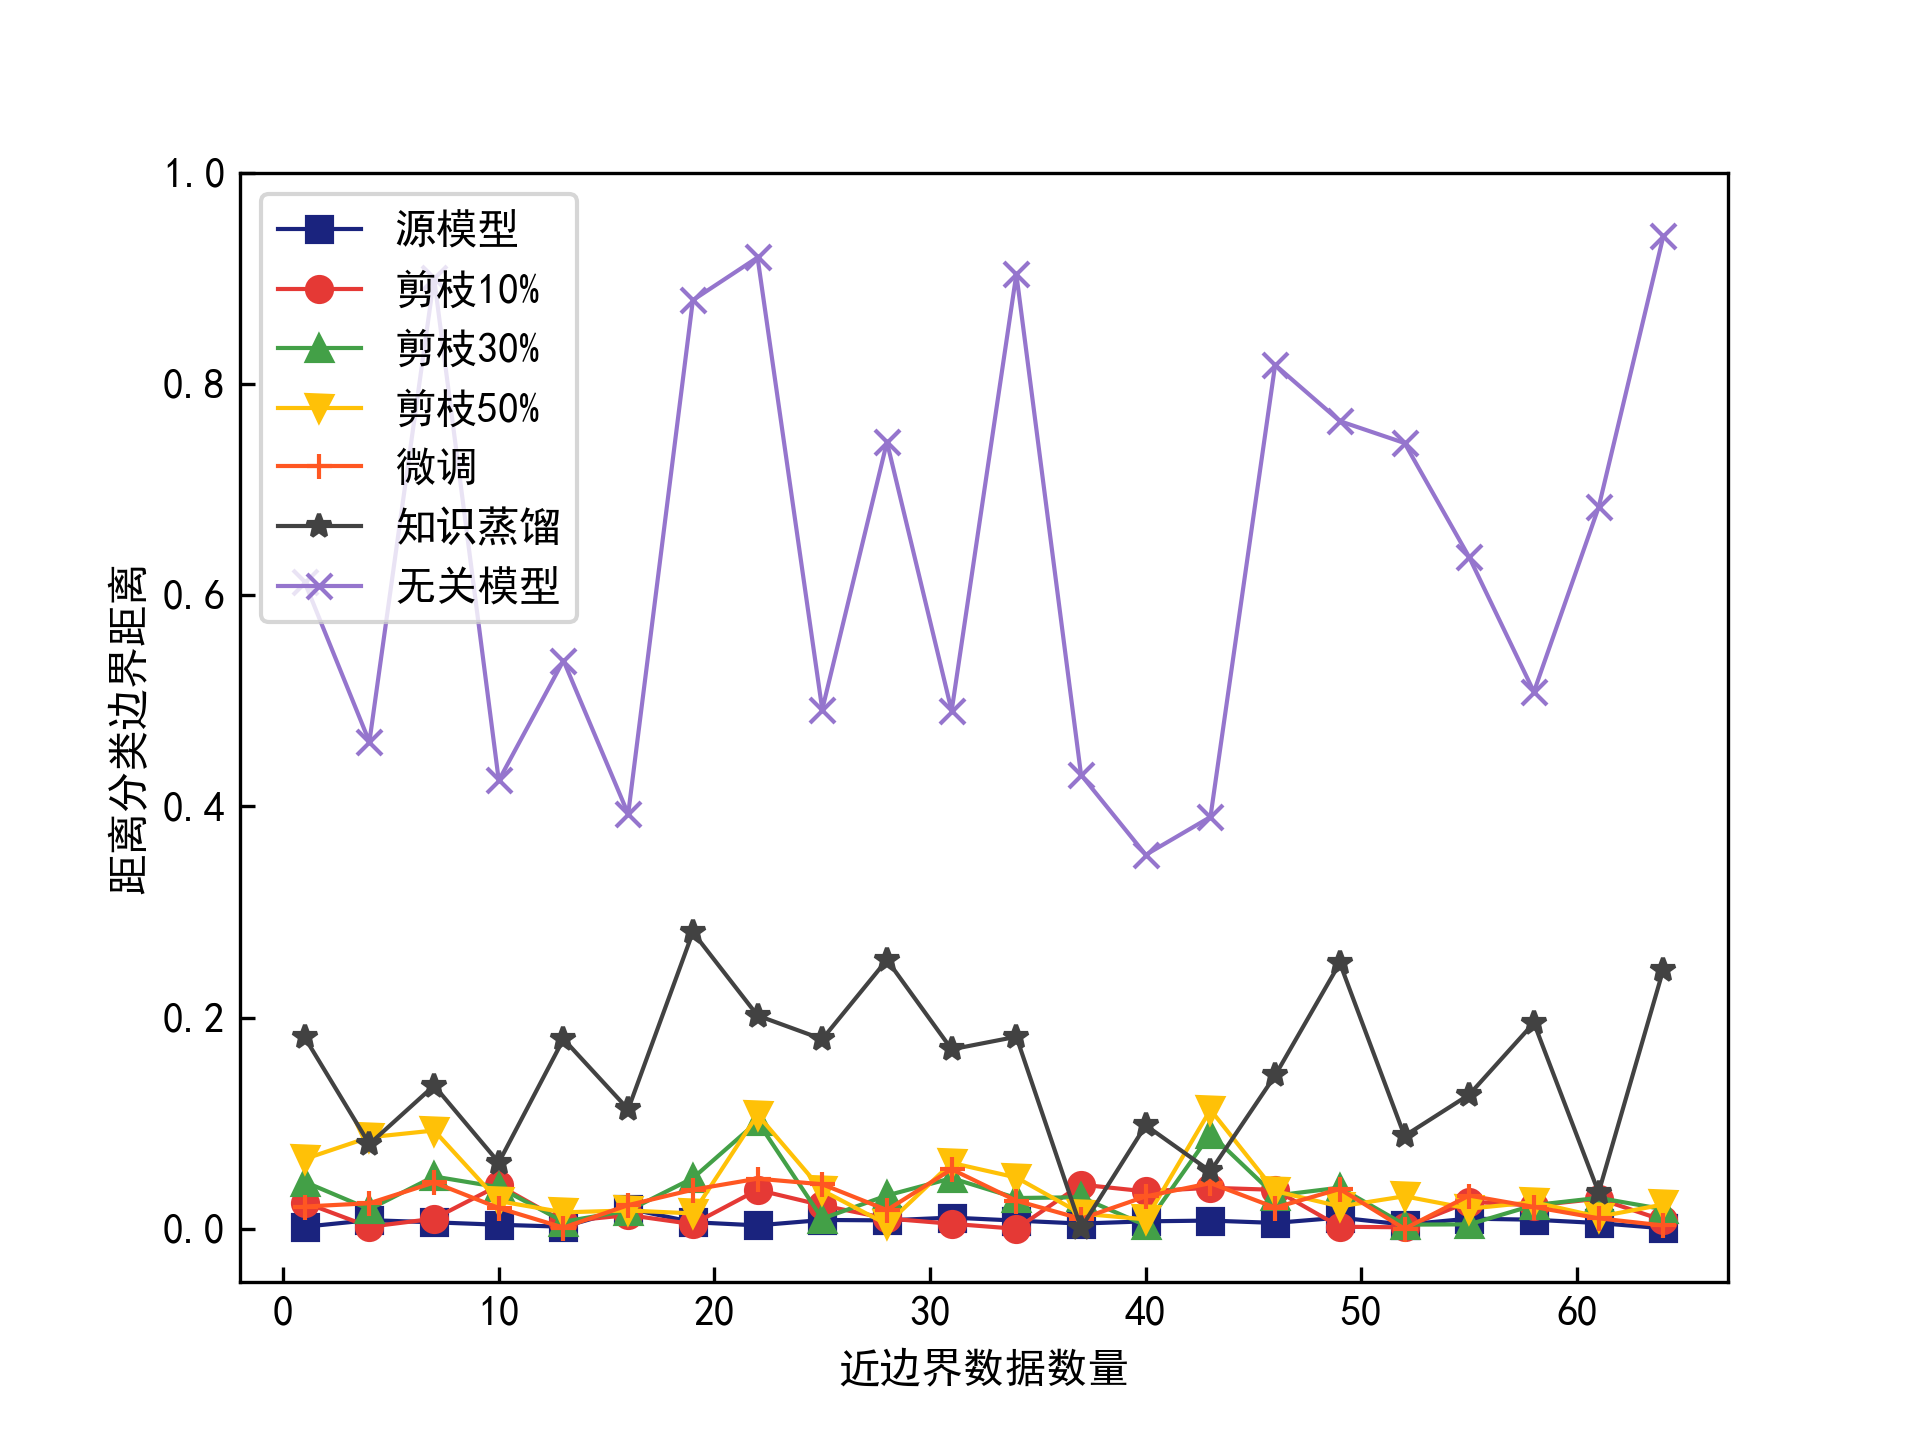
\includegraphics[width=7cm,height=4cm]{Heritage-3-0-distance.png}
		\centerline{(a)分类边界1}
	\end{minipage}
	\begin{minipage}[htbp]{0.49\linewidth}        %图片占用一行宽度的50%
		\hspace{2mm}
		\centering
		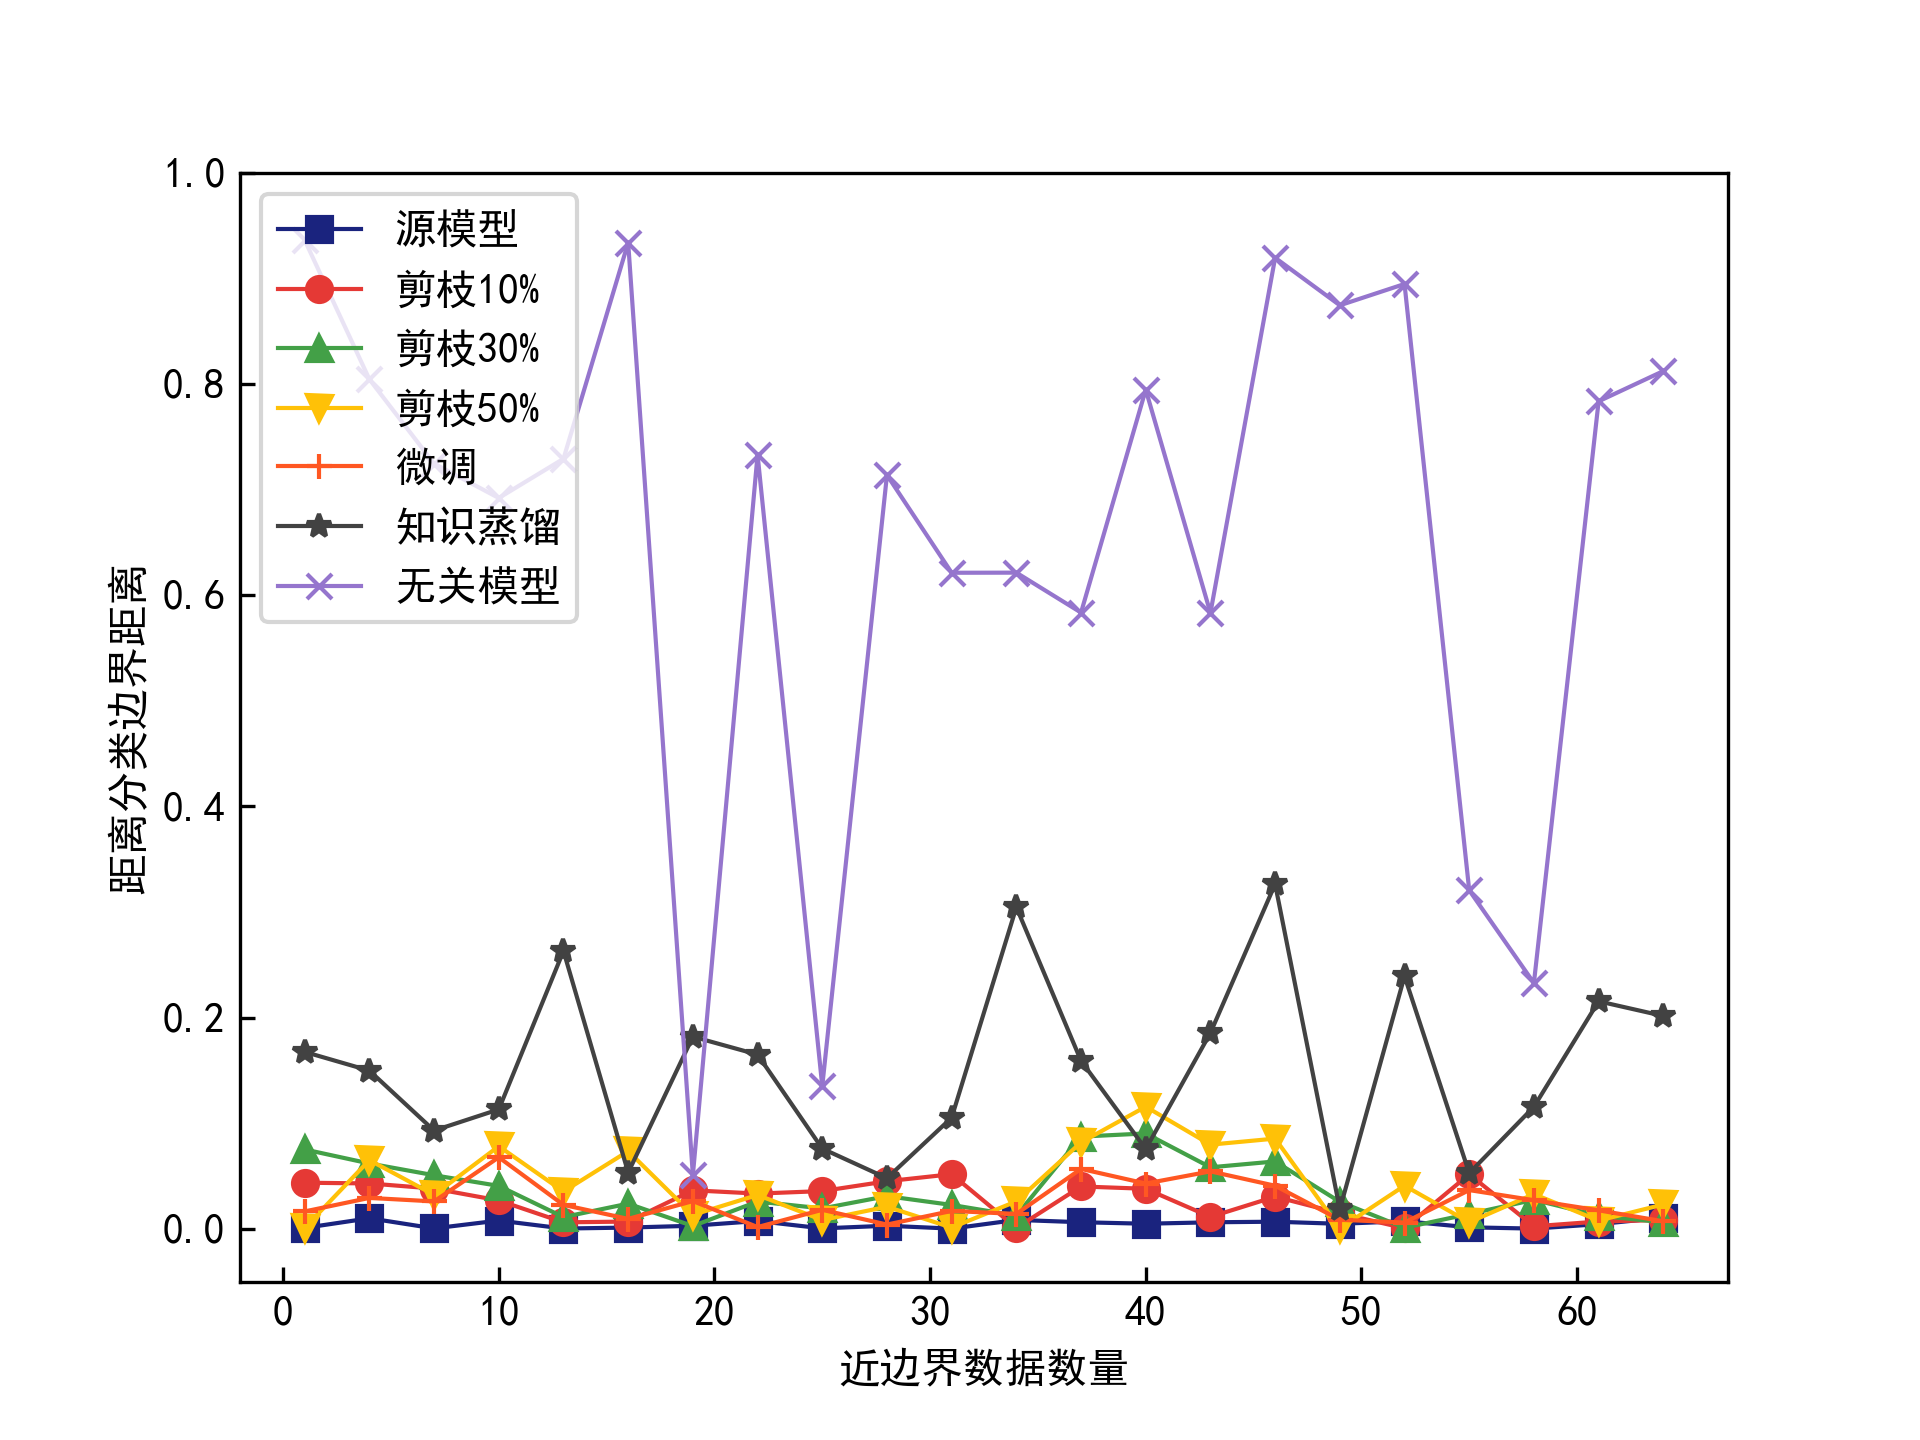
\includegraphics[width=7cm,height=4cm]{Heritage-3-1-distance.png}
		\centerline{(b)分类边界2}
	\end{minipage}
	\begin{minipage}[htbp]{0.49\linewidth}        %图片占用一行宽度的50%
		\hspace{2mm}
		\centering
		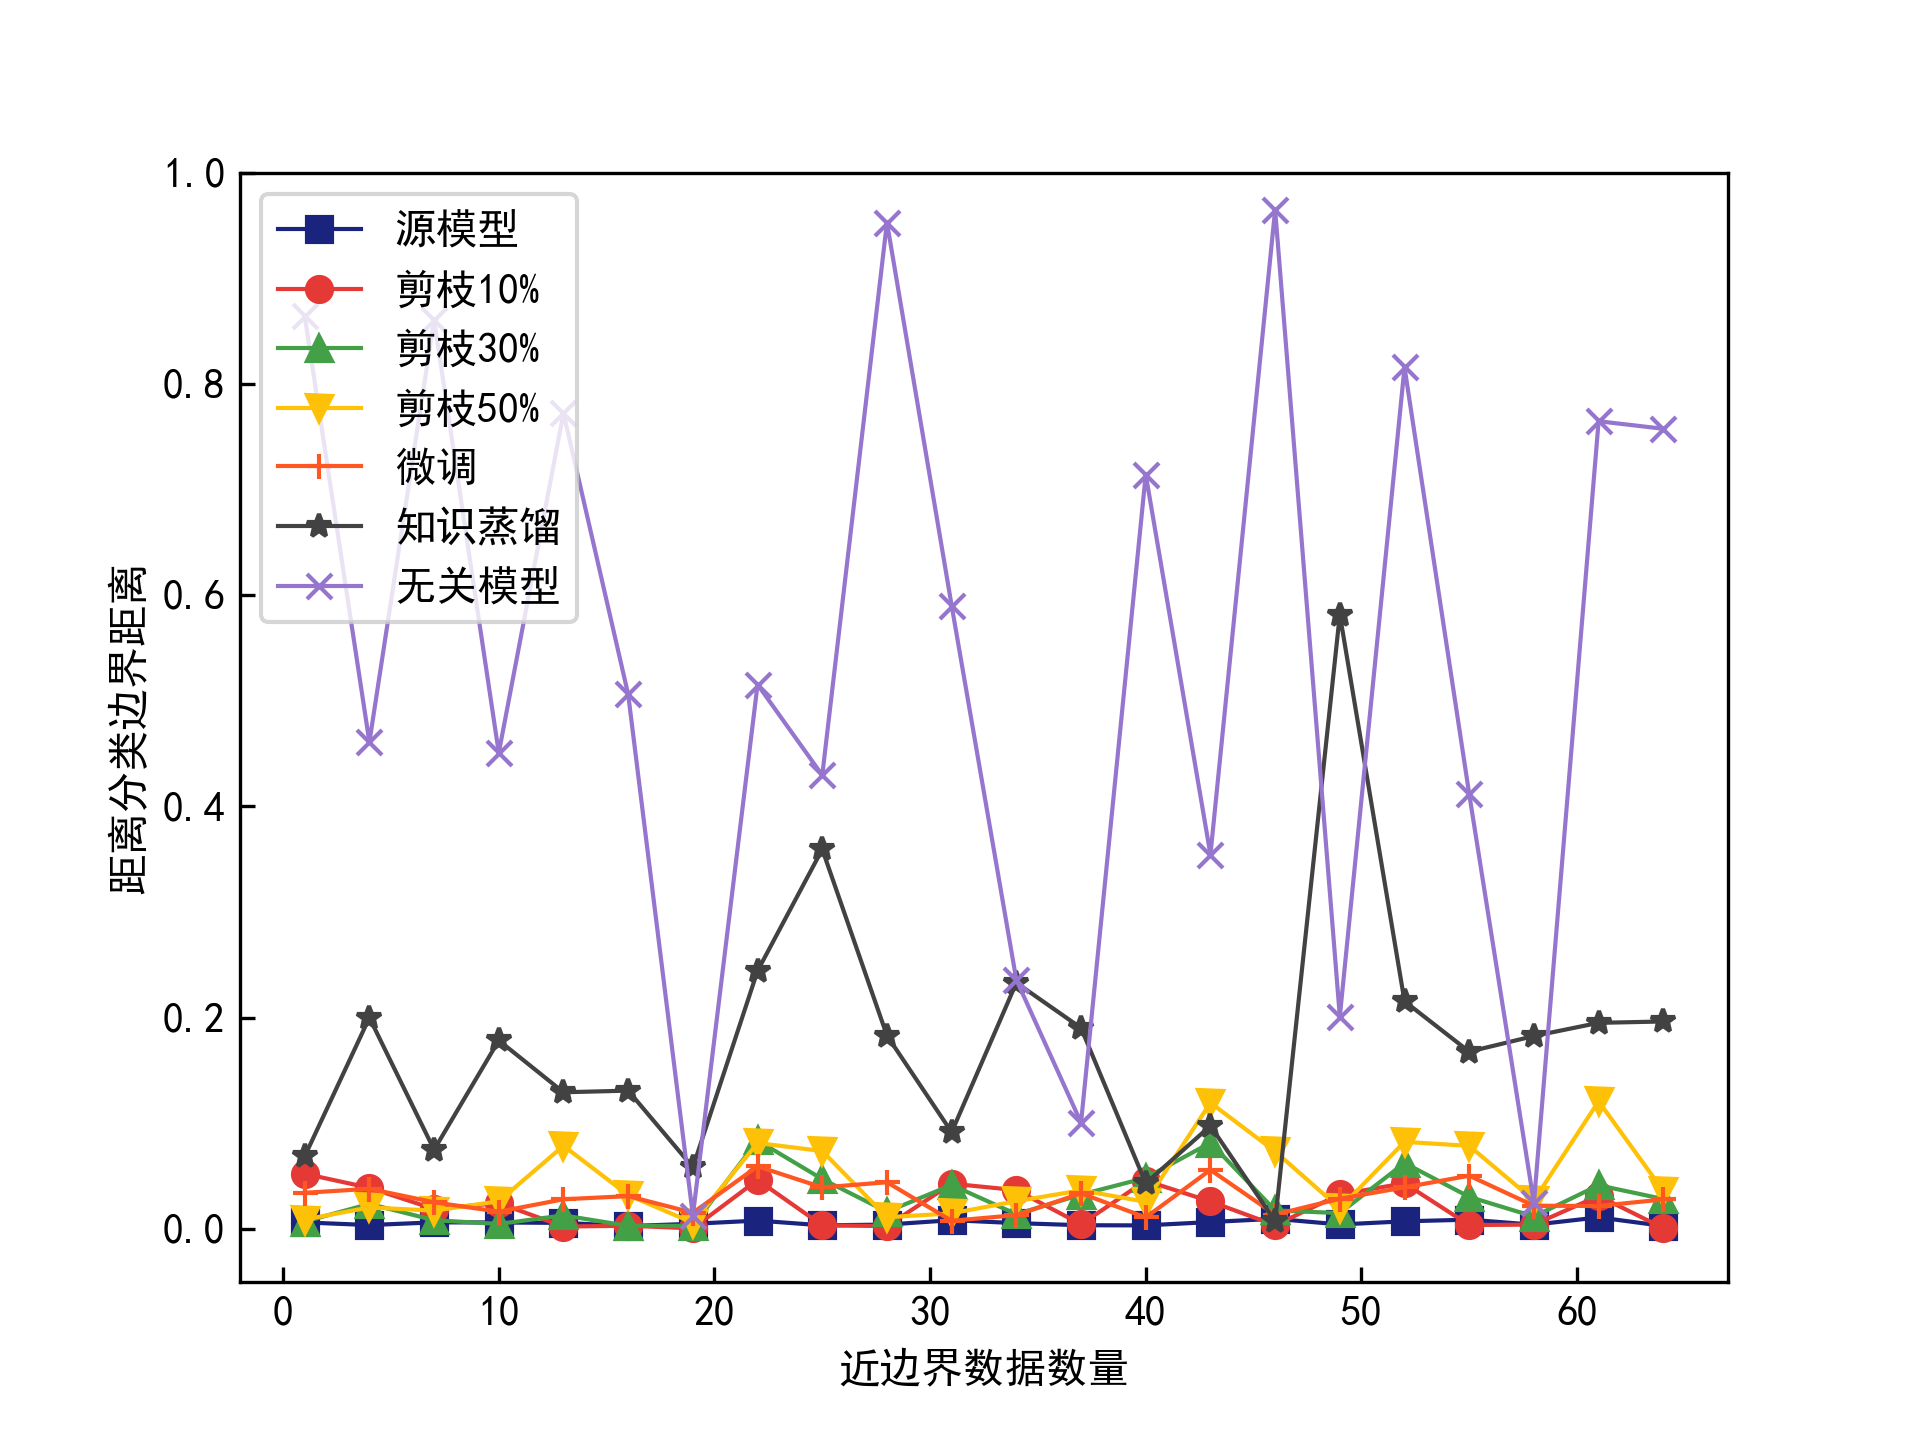
\includegraphics[width=7cm,height=4cm]{Heritage-3-4-distance.png}
		\centerline{(c)分类边界3}
	\end{minipage}
	\begin{minipage}[htbp]{0.49\linewidth}        %图片占用一行宽度的50%
		\hspace{2mm}
		\centering
		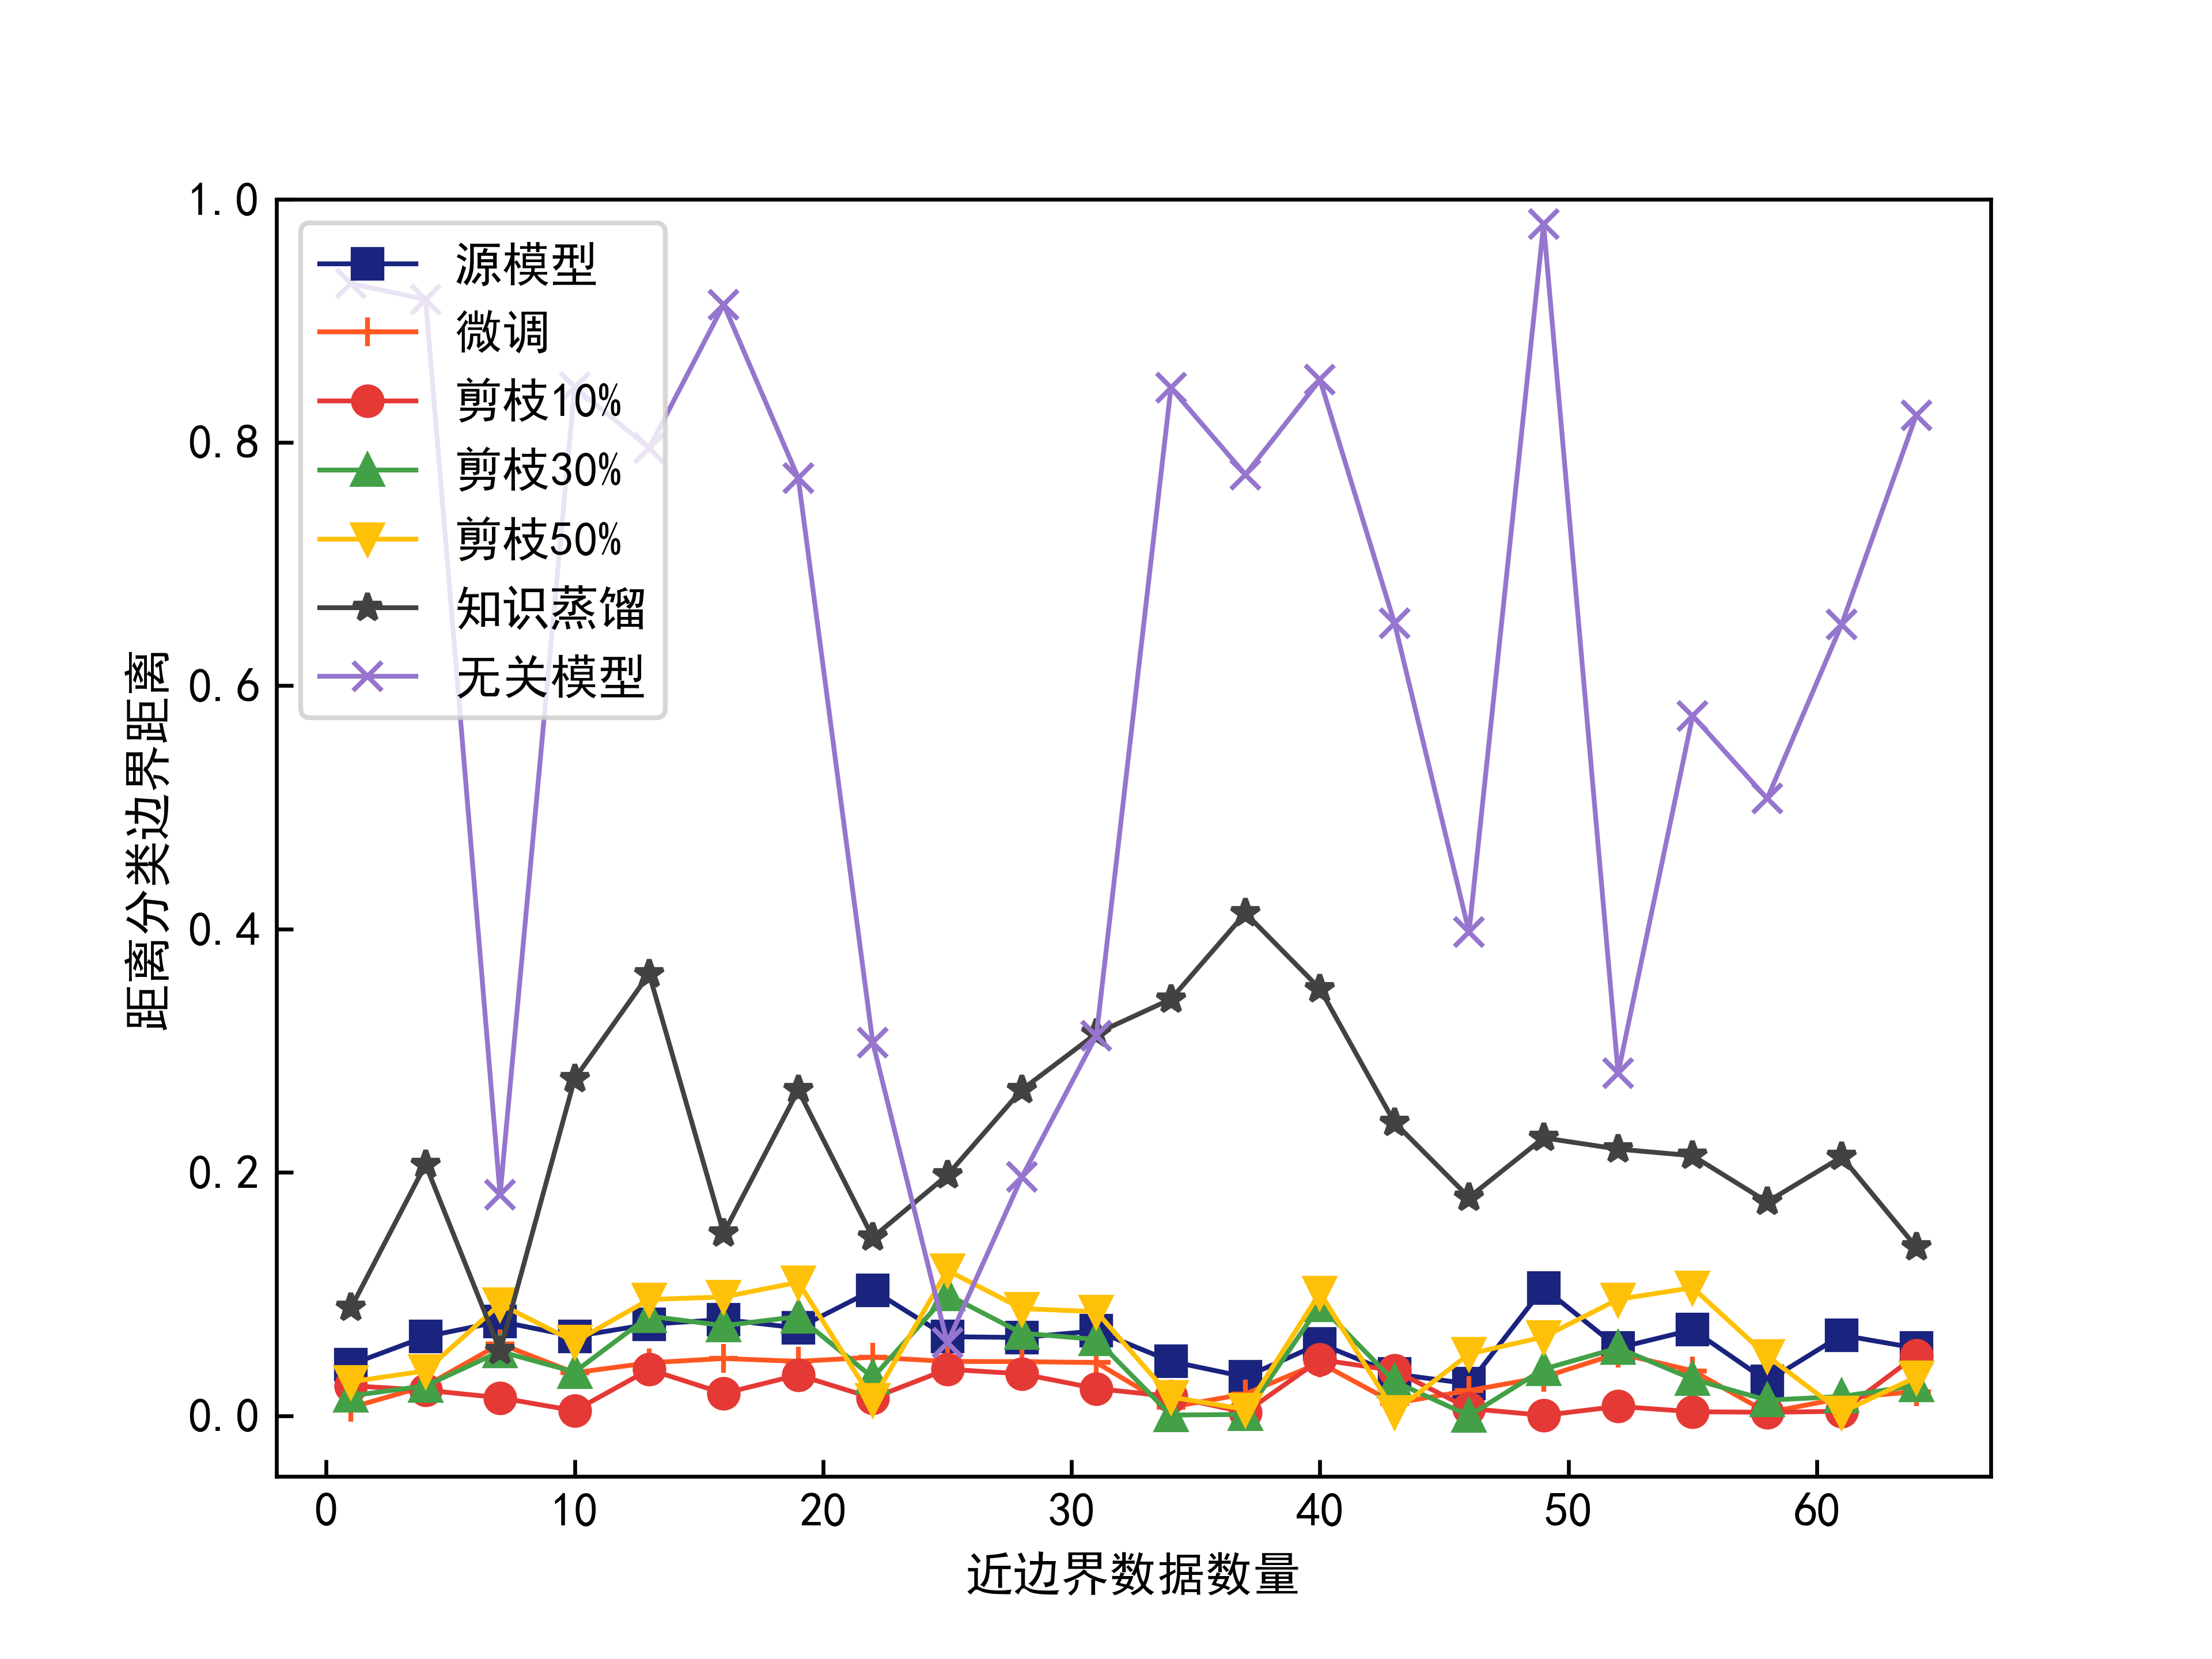
\includegraphics[width=7cm,height=4cm]{Heritage-7-6-distance.png}
		\centerline{(d)分类边界4}
	\end{minipage}
\setlength{\abovecaptionskip}{7mm} %图片标题与图片距离
\caption{Heritage上不同分类边界下的近边界数据表现}
\label{Heritage上不同分类边界下的近边界数据表现}
\end {figure}

\begin{figure}[htbp]%%图,[htbp]是浮动格式
	\centering
	\begin{minipage}[htbp]{0.49\linewidth}        %图片占用一行宽度的50%
		\hspace{2mm}
		\centering
		\includegraphics[width=7cm,height=4cm]{Intel\_image-3-1-distance.png}
		\centerline{(a)分类边界1}
	\end{minipage}
	\begin{minipage}[htbp]{0.49\linewidth}        %图片占用一行宽度的50%
		\hspace{2mm}
		\centering
		\includegraphics[width=7cm,height=4cm]{Intel\_image-3-4-distance.png}
		\centerline{(b)分类边界2}
	\end{minipage}
	\begin{minipage}[htbp]{0.49\linewidth}        %图片占用一行宽度的50%
		\hspace{2mm}
		\centering
		\includegraphics[width=7cm,height=4cm]{Intel\_image-3-5-distance.png}
		\centerline{(c)分类边界3}
	\end{minipage}
	\begin{minipage}[htbp]{0.49\linewidth}        %图片占用一行宽度的50%
		\hspace{2mm}
		\centering
		\includegraphics[width=7cm,height=4cm]{Intel\_image-5-0-distance.png}
		\centerline{(d)分类边界4}
	\end{minipage}
\setlength{\abovecaptionskip}{7mm} %图片标题与图片距离
\caption{Intel\_image上不同分类边界下的近边界数据表现}
\label{Intel-image上不同分类边界下的近边界数据表现}
\end {figure}
	
\section{推断模型所有权}\label{5.4}

在本节中,我们讨论了我们方法在与其他近边界数据在盗窃模型上的性能对比,我们模拟了盗窃者可能会提供的近边界数据,该数据由几部分组成,包括(1)从原始数据中挑选出的近边界数据,(2)由FGSM和CW生成的一些对抗性样本。我们针对不同的目标分类边界,按照\ref{4.2.3}中进行假设检验并计算在不同数据集和不同盗窃模型上的$\Delta\mu$和$p$值。如表\ref{table:2}所示,$p$值显著低于0.05在全部情况中。换句话说,我们的方法在不同的盗窃方法中推断模型所有权均有显著的效果。尽管在模型蒸馏上表现不如其他情况。实验结果表明使用私有的近边界数据对大多数模型盗窃技术都是可靠的,我们可以声称模型被盗窃的置信度至少为95\%,模型蒸馏是我们方法的最大挑战,也同样是其他研究面临的巨大挑战,在我们的实验中,可以观察到我们的模型始终可以将蒸馏模型标记为被盗的模型,这证明了我们方法的鲁棒性。


\begin{table}[H]
	\centering
	\setlength{\arrayrulewidth}{0.5mm}
	\renewcommand\arraystretch{1.5}
	\caption{推断模型所有权}
	\label{table:2}
	\resizebox{\linewidth}{!}{
	\begin{tabular}{l l c c c c c c c c c c}
		
		\hline
\multirow{2}{5em}{数据集}&\multirow{2}{4em}{攻击方法}&\multicolumn{2}{c}{分类边界1}&\multicolumn{2}{c}{分类边界2}&\multicolumn{2}{c}{分类边界3}&\multicolumn{2}{c}{分类边界4}&\multicolumn{2}{c}{分类边界5}\\ \cline{3-12}
		                         & &$\Delta\mu$&$p$值&$\Delta\mu$&$p$值&$\Delta\mu$&$p$值&$\Delta\mu$&$p$值&$\Delta\mu$&$p$值 \\
		\hline
\multirow{6}{5em}{CIFAR-10}     &源模型    & 0.913 & $10^{-6}$ & 0.954 & $10^{-6}$ & 0.927 & $10^{-5}$ & 0.967 & $10^{-5}$ & 0.958 & $10^{-5}$   \\
								&模型微调  & 0.718 & $10^{-5}$ & 0.745 & $10^{-6}$ & 0.698 & $10^{-5}$ & 0.692 & $10^{-4}$ & 0.729 & $10^{-5}$   \\
								& 剪枝10\% & 0.572 & $10^{-5}$ & 0.487 & $10^{-5}$ & 0.458 & $10^{-5}$ & 0.533 & $10^{-4}$ & 0.512 & $10^{-4}$   \\
								&剪枝30\%  & 0.537 & $10^{-4}$ & 0.497 & $10^{-4}$ & 0.401 & $10^{-3}$ & 0.428 & $10^{-4}$ & 0.587 & $10^{-4}$   \\
								&剪枝50\%  & 0.545 & $10^{-4}$ & 0.614 & $10^{-4}$ & 0.506 & $10^{-3}$ & 0.570 & $10^{-4}$ & 0.484 & $10^{-3}$   \\
								&知识蒸馏  & 0.372 & $10^{-3}$ & 0.297 & $10^{-3}$ & 0.288 & $10^{-3}$ & 0.308 & $10^{-3}$ & 0.340 & $10^{-3}$   \\
		\hline
\multirow{6}{5em}{Heritage}     &源模型    & 0.876 & $10^{-5}$ & 0.845 & $10^{-5}$ & 0.859 & $10^{-4}$ & 0.801 & $10^{-4}$ & 0.837 & $10^{-5}$   \\
								&模型微调  & 0.815 & $10^{-5}$ & 0.792 & $10^{-4}$ & 0.824 & $10^{-4}$ & 0.833 & $10^{-4}$ & 0.784 & $10^{-4}$   \\
								&剪枝10\%  & 0.530 & $10^{-4}$ & 0.535 & $10^{-3}$ & 0.508 & $10^{-4}$ & 0.486 & $10^{-3}$ & 0.471 & $10^{-3}$   \\
								&剪枝30\%  & 0.491 & $10^{-3}$ & 0.452 & $10^{-3}$ & 0.469 & $10^{-4}$ & 0.470 & $10^{-3}$ & 0.427 & $10^{-4}$   \\
								&剪枝50\%  & 0.502 & $10^{-3}$ & 0.517 & $10^{-3}$ & 0.434 & $10^{-3}$ & 0.451 & $10^{-3}$ & 0.490 & $10^{-3}$   \\
								&知识蒸馏  & 0.329 & $10^{-3}$ & 0.365 & $10^{-2}$ & 0.238 & $10^{-3}$ & 0.310 & $10^{-3}$ & 0.274 & $10^{-3}$   \\
		\hline
\multirow{6}{5em}{Intel\_image} &源模型    & 0.859 & $10^{-5}$ & 0.896 & $10^{-4}$ & 0.872 & $10^{-4}$ & 0.899 & $10^{-4}$ & 0.914 & $10^{-4}$   \\
								&模型微调  & 0.717 & $10^{-5}$ & 0.784 & $10^{-4}$ & 0.752 & $10^{-4}$ & 0.791 & $10^{-3}$ & 0.709 & $10^{-4}$   \\
								&剪枝10\%  & 0.451 & $10^{-4}$ & 0.522 & $10^{-4}$ & 0.539 & $10^{-3}$ & 0.472 & $10^{-3}$ & 0.438 & $10^{-4}$   \\
								&剪枝30\%  & 0.407 & $10^{-4}$ & 0.415 & $10^{-4}$ & 0.346 & $10^{-3}$ & 0.382 & $10^{-3}$ & 0.395 & $10^{-3}$   \\
								&剪枝50\%  & 0.370 & $10^{-3}$ & 0.395 & $10^{-3}$ & 0.327 & $10^{-3}$ & 0.360 & $10^{-3}$ & 0.458 & $10^{-3}$   \\
								&知识蒸馏  & 0.336 & $10^{-2}$ & 0.395 & $10^{-3}$ & 0.360 & $10^{-2}$ & 0.308 & $10^{-3}$ & 0.287 & $10^{-2}$   \\
		\hline		
	\end{tabular}
}
\end{table}



\section{微调目标分类边界的影响}\label{5.5}

本小节对\ref{3}\ref{3.3}中测试微调对源模型的影响进行了广泛的实验。我们针对不同数据集训练得到的源模型,使用不同规模的近边界数据以及不同的目标分类边界对源模型进行微调。如表\ref{table:3}表\ref{table:4}表\ref{table:5}所示,几乎全部情况下的源模型微调前后精度差均不超过5pp。实验结果证明,我们的近边界数据在应用于模型所有权保护问题中,具有较好的保真度。因此,使用近边界数据推断模型所有权不用担心源模型受到较大的影响。

\begin{table}[H]
	\centering
	\setlength{\arrayrulewidth}{0.5mm}
	\renewcommand\arraystretch{1.2}
	\caption{CIFAR-10上不同对抗性样本生成算法生成的数据与目标分类边界的平均距离}
	\label{table:3}
	\begin{tabular*}{14cm}{@{\extracolsep{\fill}} l l c c}
		
		\hline
		数据集 \ (准确率)   &   分类边界   &  数据数量  &   微调后准确率    \\
		\hline
\multirow{20}{8em}{CIFAR-10\ (0.886)}         &\multirow{4}{6em}{分类边界1}&  64   & 0.873    \\
								              &                           &  128  & 0.862     \\
								              &                           &  256  & 0.862     \\
								              &                           &  512  & 0.854     \\
		\cline{2-4}						   
								              &\multirow{4}{6em}{分类边界2} &  64  & 0.871 \\
								              &                            &  128 & 0.870     \\
								              &                            &  256 & 0.860     \\
								              &                            &  512 & 0.844     \\
		
		\cline{2-4}						       
											  &\multirow{4}{6em}{分类边界3} & 64   & 0.871  \\
											  &                            &  128 & 0.868     \\
											  &                            &  256 & 0.858     \\
											  &                            &  512 & 0.856     \\
		\cline{2-4}						       
											  &\multirow{4}{6em}{分类边界4} & 64   & 0.873  \\
											  &                            &  128 & 0.873     \\
											  &                            &  256 & 0.866     \\
											  &                            &  512 & 0.862     \\
		\cline{2-4}						       
											  &\multirow{4}{6em}{分类边界5} & 64  & 0.876  \\
											  &                            & 128 & 0.866     \\
											  &                            & 256 & 0.868     \\
											  &                            & 512 & 0.861     \\
		\hline	
	\end{tabular*}
\end{table}


\begin{table}[H]
	\centering
	\setlength{\arrayrulewidth}{0.5mm}
	\renewcommand\arraystretch{1.2}
	\caption{Heritage上不同对抗性样本生成算法生成的数据与目标分类边界的平均距离}
	\label{table:4}
	\begin{tabular*}{14cm}{@{\extracolsep{\fill}} l l c c}
		
		\hline
		数据集 \ (准确率)   &   分类边界   &  数据数量  &   微调后准确率    \\
		\hline
		\multirow{20}{8em}{Heritage\ (0.879)}         &\multirow{4}{6em}{分类边界1}&  64   & 0.856    \\
		&                           &  128  & 0.825     \\
		&                           &  256  & 0.830     \\
		&                           &  512  & 0.797     \\
		\cline{2-4}						   
		&\multirow{4}{6em}{分类边界2} &  64  & 0.823 \\
		&                            &  128 & 0.839     \\
		&                            &  256 & 0.841     \\
		&                            &  512 & 0.779     \\
		
		\cline{2-4}						       
		&\multirow{4}{6em}{分类边界3} & 64   & 0.848  \\
		&                            &  128 & 0.826     \\
		&                            &  256 & 0.779     \\
		&                            &  512 & 0.791     \\
		\cline{2-4}						       
		&\multirow{4}{6em}{分类边界4} & 64   & 0.819  \\
		&                            &  128 & 0.795     \\
		&                            &  256 & 0.803     \\
		&                            &  512 & 0.783     \\
		\cline{2-4}						       
		&\multirow{4}{6em}{分类边界5} & 64  & 0.843  \\
		&                            & 128 & 0.851     \\
		&                            & 256 & 0.776     \\
		&                            & 512 & 0.774     \\
		\hline	
	\end{tabular*}
\end{table}

\begin{table}[H]
	\centering
	\setlength{\arrayrulewidth}{0.5mm}
	\renewcommand\arraystretch{1.2}
	\caption{Intel\_image上不同对抗性样本生成算法生成的数据与目标分类边界的平均距离}
	\label{table:5}
	\begin{tabular*}{14cm}{@{\extracolsep{\fill}} l l c c}
		
		\hline
		数据集 \ (准确率)   &   分类边界   &  数据数量  &   微调后准确率    \\
		\hline
		\multirow{20}{8em}{Intel\_image\ (0.794)}    &\multirow{4}{6em}{分类边界1}&  64   & 0.755    \\
		&                           &  128  & 0.769     \\
		&                           &  256  & 0.756     \\
		&                           &  512  & 0.779     \\
		\cline{2-4}						   
		&\multirow{4}{6em}{分类边界2} &  64  & 0.770 \\
		&                            &  128 & 0.741     \\
		&                            &  256 & 0.768     \\
		&                            &  512 & 0.777     \\
		
		\cline{2-4}						       
		&\multirow{4}{6em}{分类边界3} &  64  & 0.781  \\
		&                            &  128 & 0.753     \\
		&                            &  256 & 0.764     \\
		&                            &  512 & 0.752     \\
		\cline{2-4}						       
		&\multirow{4}{6em}{分类边界4} & 64   & 0.787  \\
		&                            &  128 & 0.751     \\
		&                            &  256 & 0.762     \\
		&                            &  512 & 0.747     \\
		\cline{2-4}						       
		&\multirow{4}{6em}{分类边界5} & 64  & 0.786  \\
		&                            & 128 & 0.764     \\
		&                            & 256 & 0.761     \\
		&                            & 512 & 0.765     \\
		\hline	
	\end{tabular*}
\end{table}

\section{可伸缩性扩展}\label{5.6}

在本节中,我们测试了不同规模的近边界数据在推断模型所有权上的可伸缩性。回想我们的方法需要对数据进行采样从而进行假设检验,通常来说样本数量越大,对检验过程中因随机而产生的不利影响越少,在推断所有权上越有信心。如图\ref{CIFAR-10上推断模型所有权的扩展性}图\ref{Heritage上推断模型所有权的扩展性}图\ref{Intel-image上推断模型所有权的扩展性}所示,$p$值随着近边界数据的规模增大而减少,也就是说近边界数据越多推断的信心也越多,但这并不说明我们的方法对小数量的近边界数据缺少鲁棒性,从表中我们可以观察到即使数据量为64 的情况下,$p$值仍小于0.05,这证明我们的方法对于小数量同样有显著的效果。

\begin{figure}[htbp]%%图,[htbp]是浮动格式
	\centering
	\begin{minipage}[htbp]{0.49\linewidth}        %图片占用一行宽度的50%
		\hspace{2mm}
		\centering
		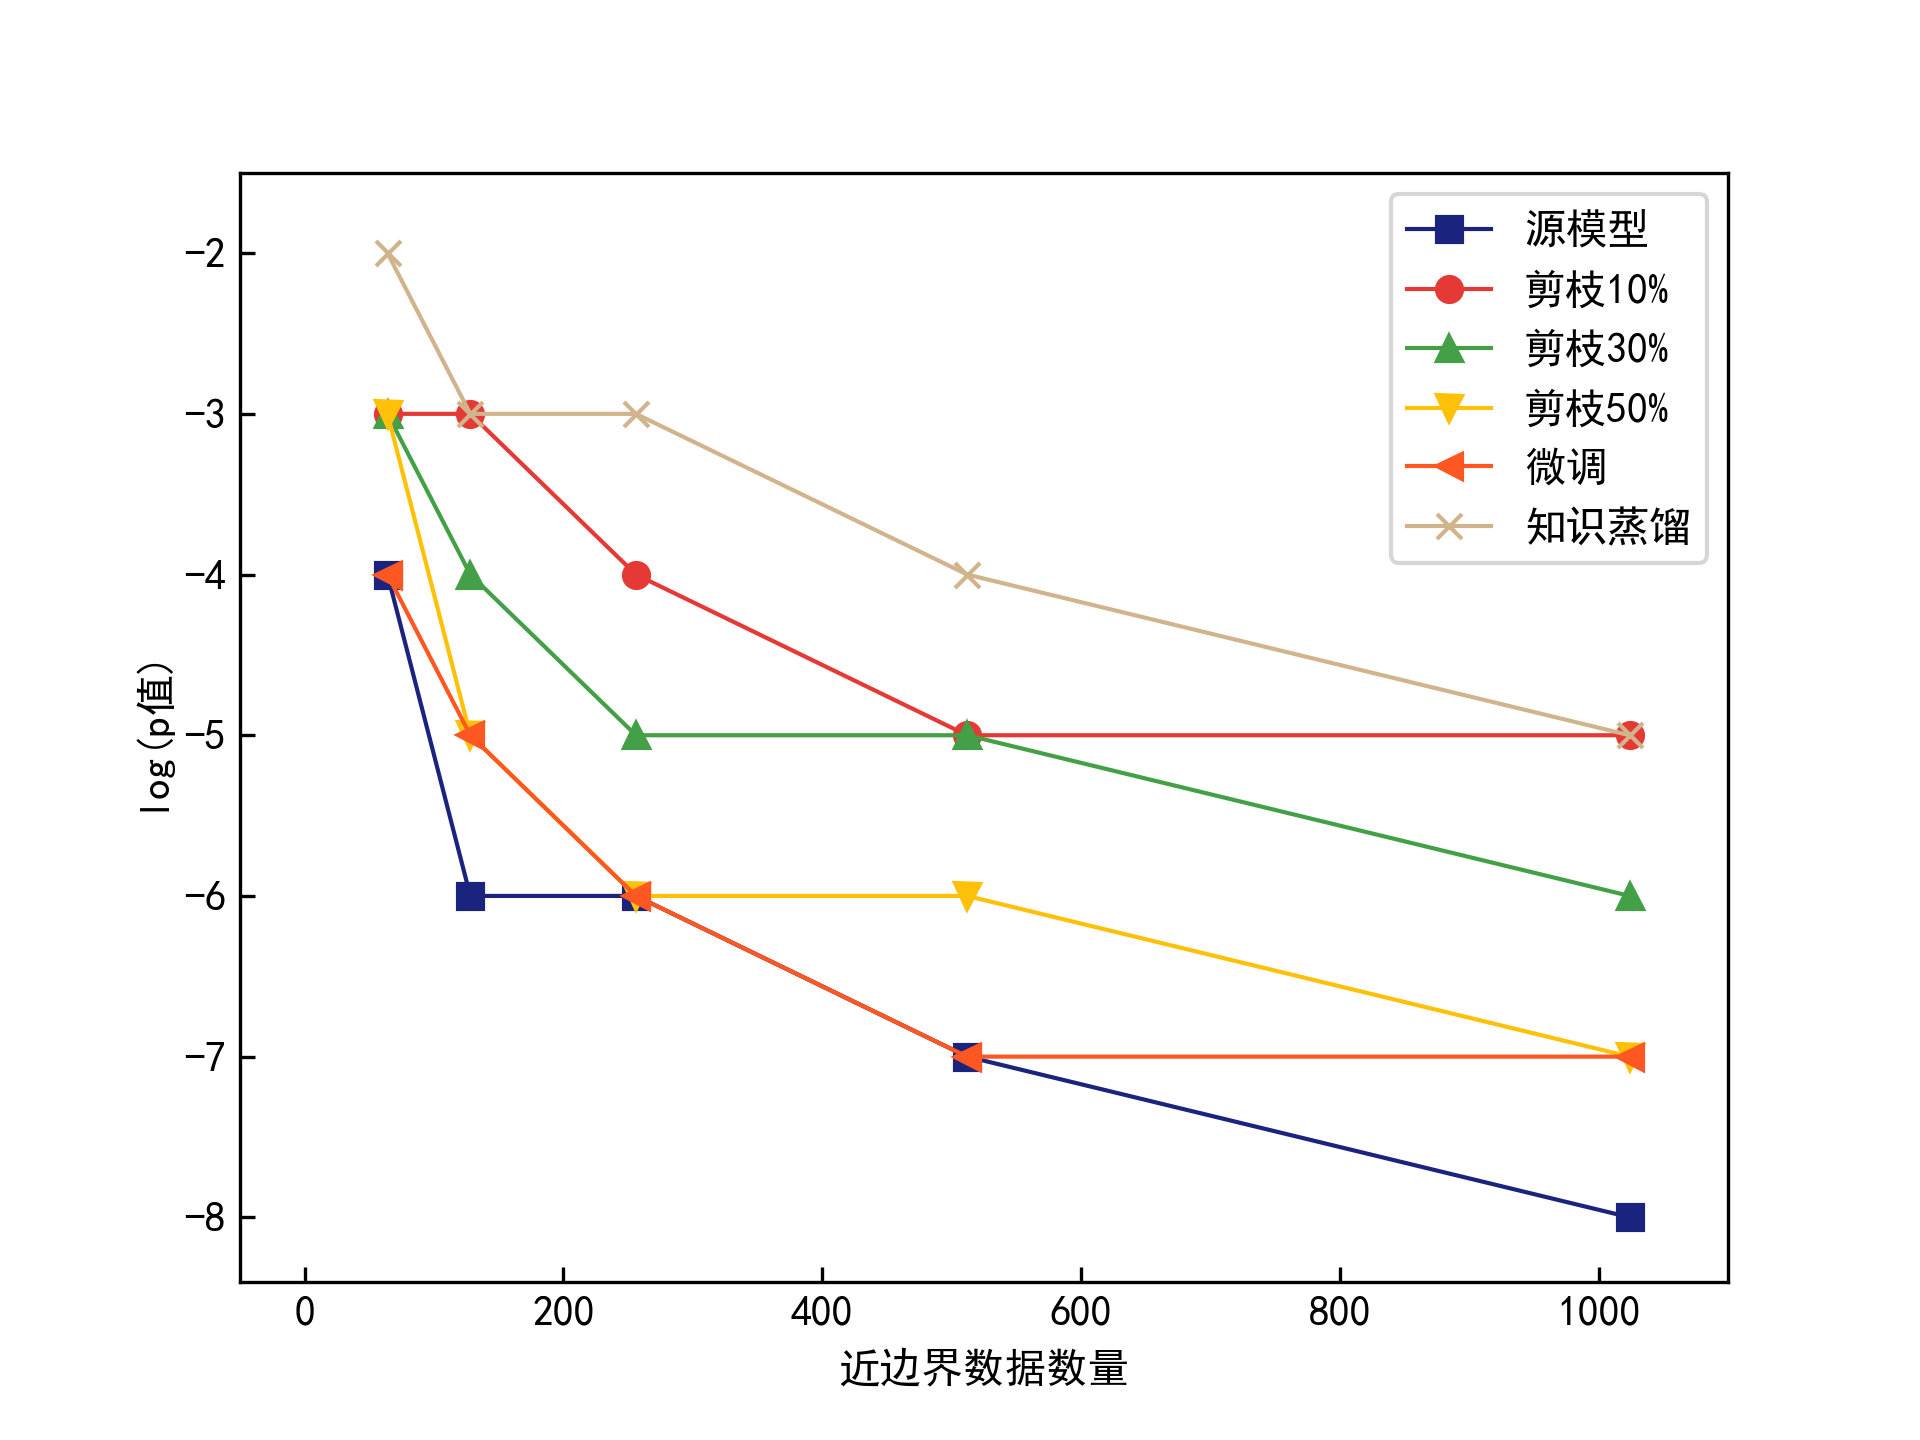
\includegraphics[width=7cm,height=4cm]{CIFAR-10-4-2-p-value.png}
		\centerline{(a)分类边界1}
	\end{minipage}
	\begin{minipage}[htbp]{0.49\linewidth}        %图片占用一行宽度的50%
		\hspace{2mm}
		\centering
		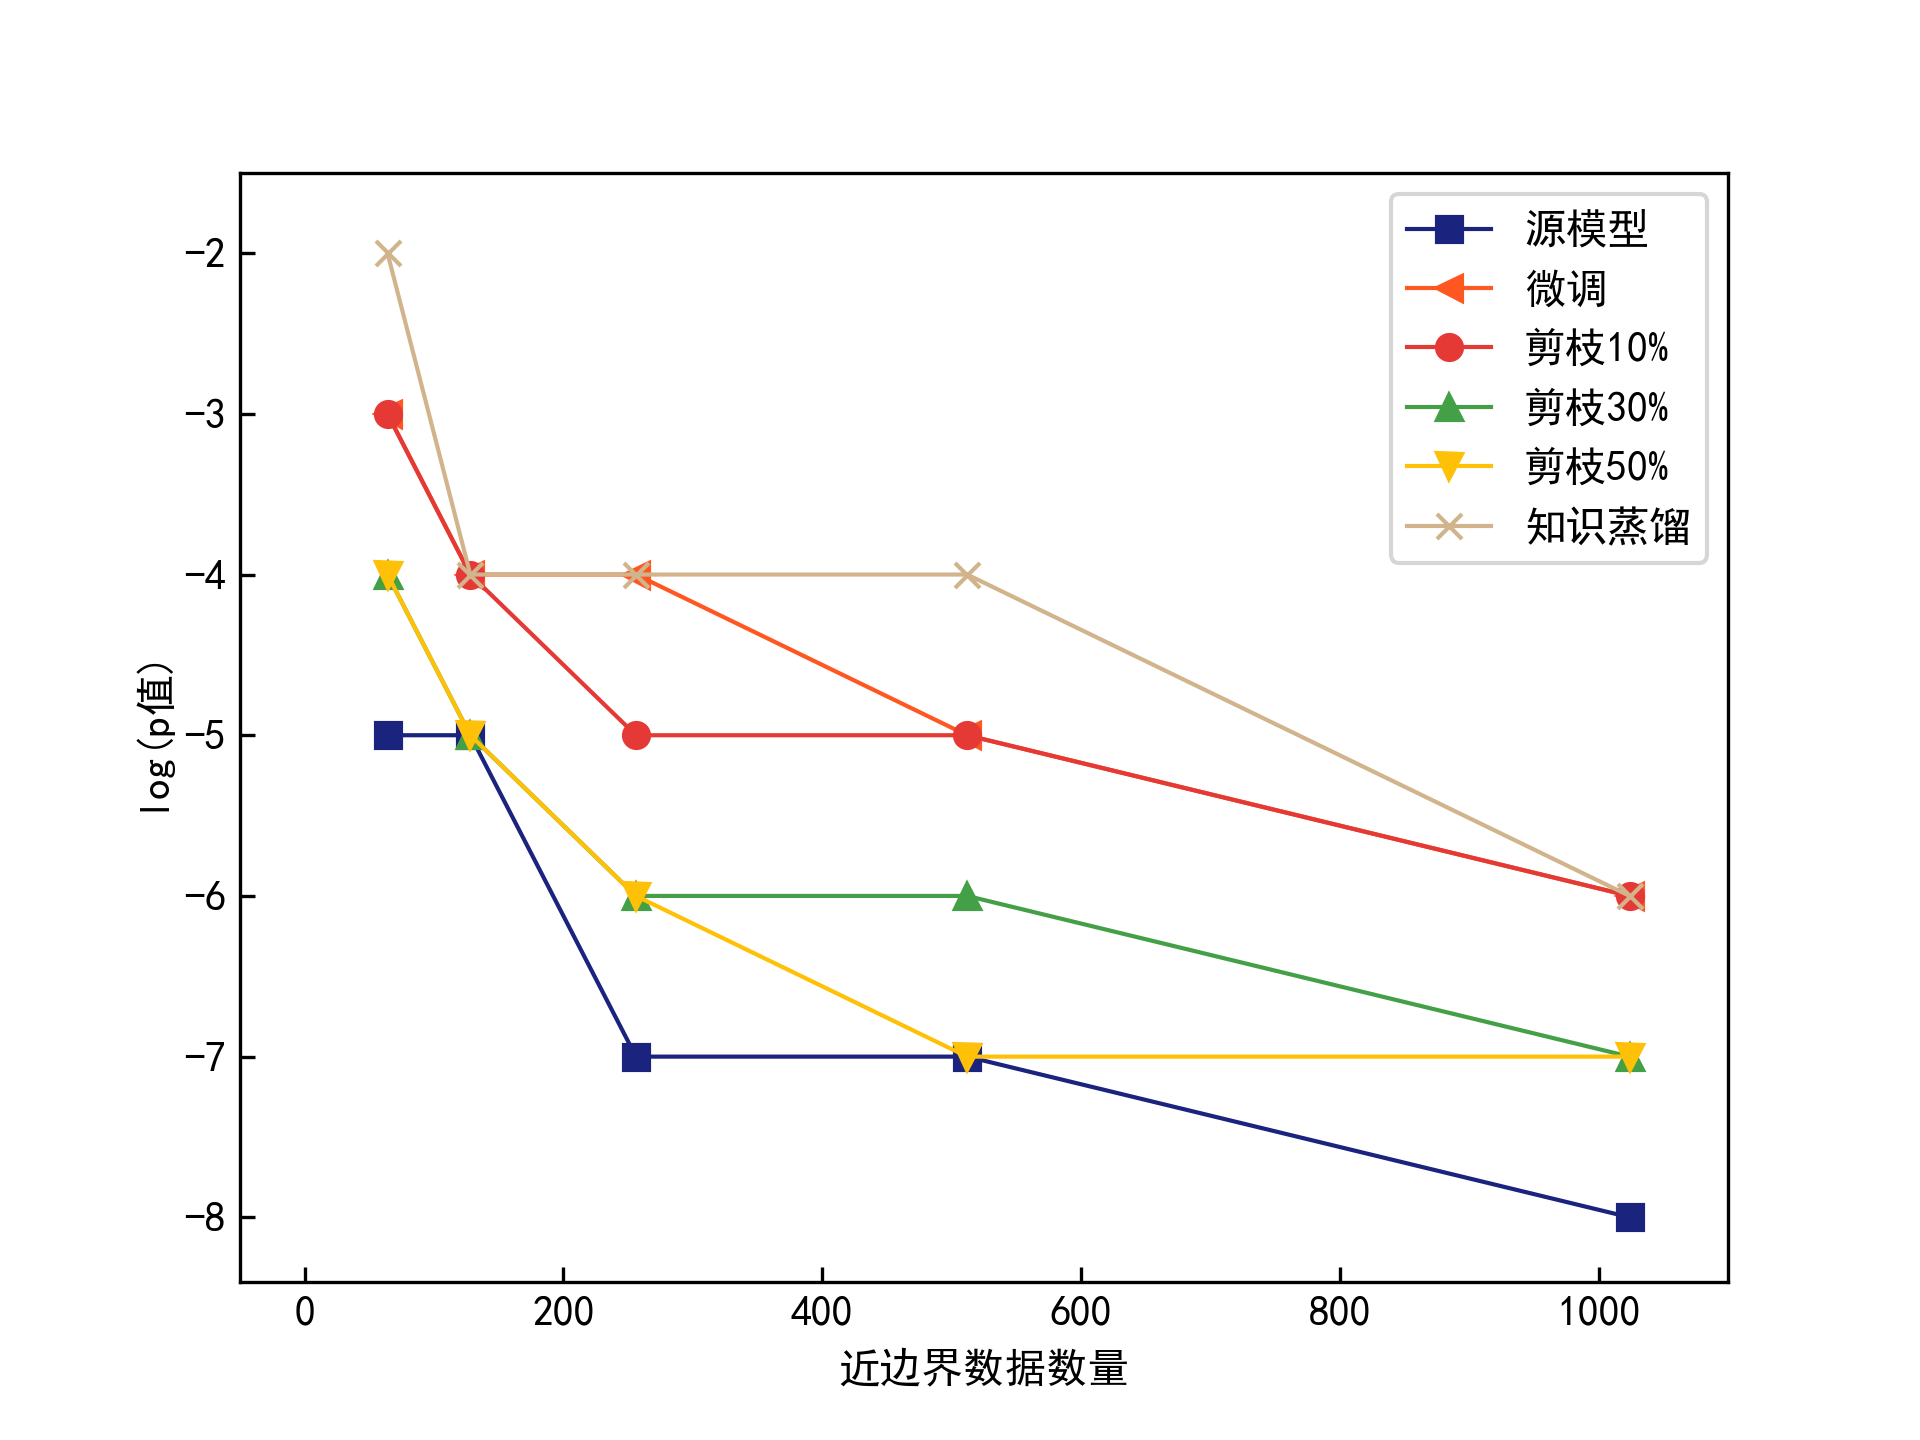
\includegraphics[width=7cm,height=4cm]{CIFAR-10-4-3-p-value.png}
		\centerline{(b)分类边界2}
	\end{minipage}
	\begin{minipage}[htbp]{0.49\linewidth}        %图片占用一行宽度的50%
		\hspace{2mm}
		\centering
		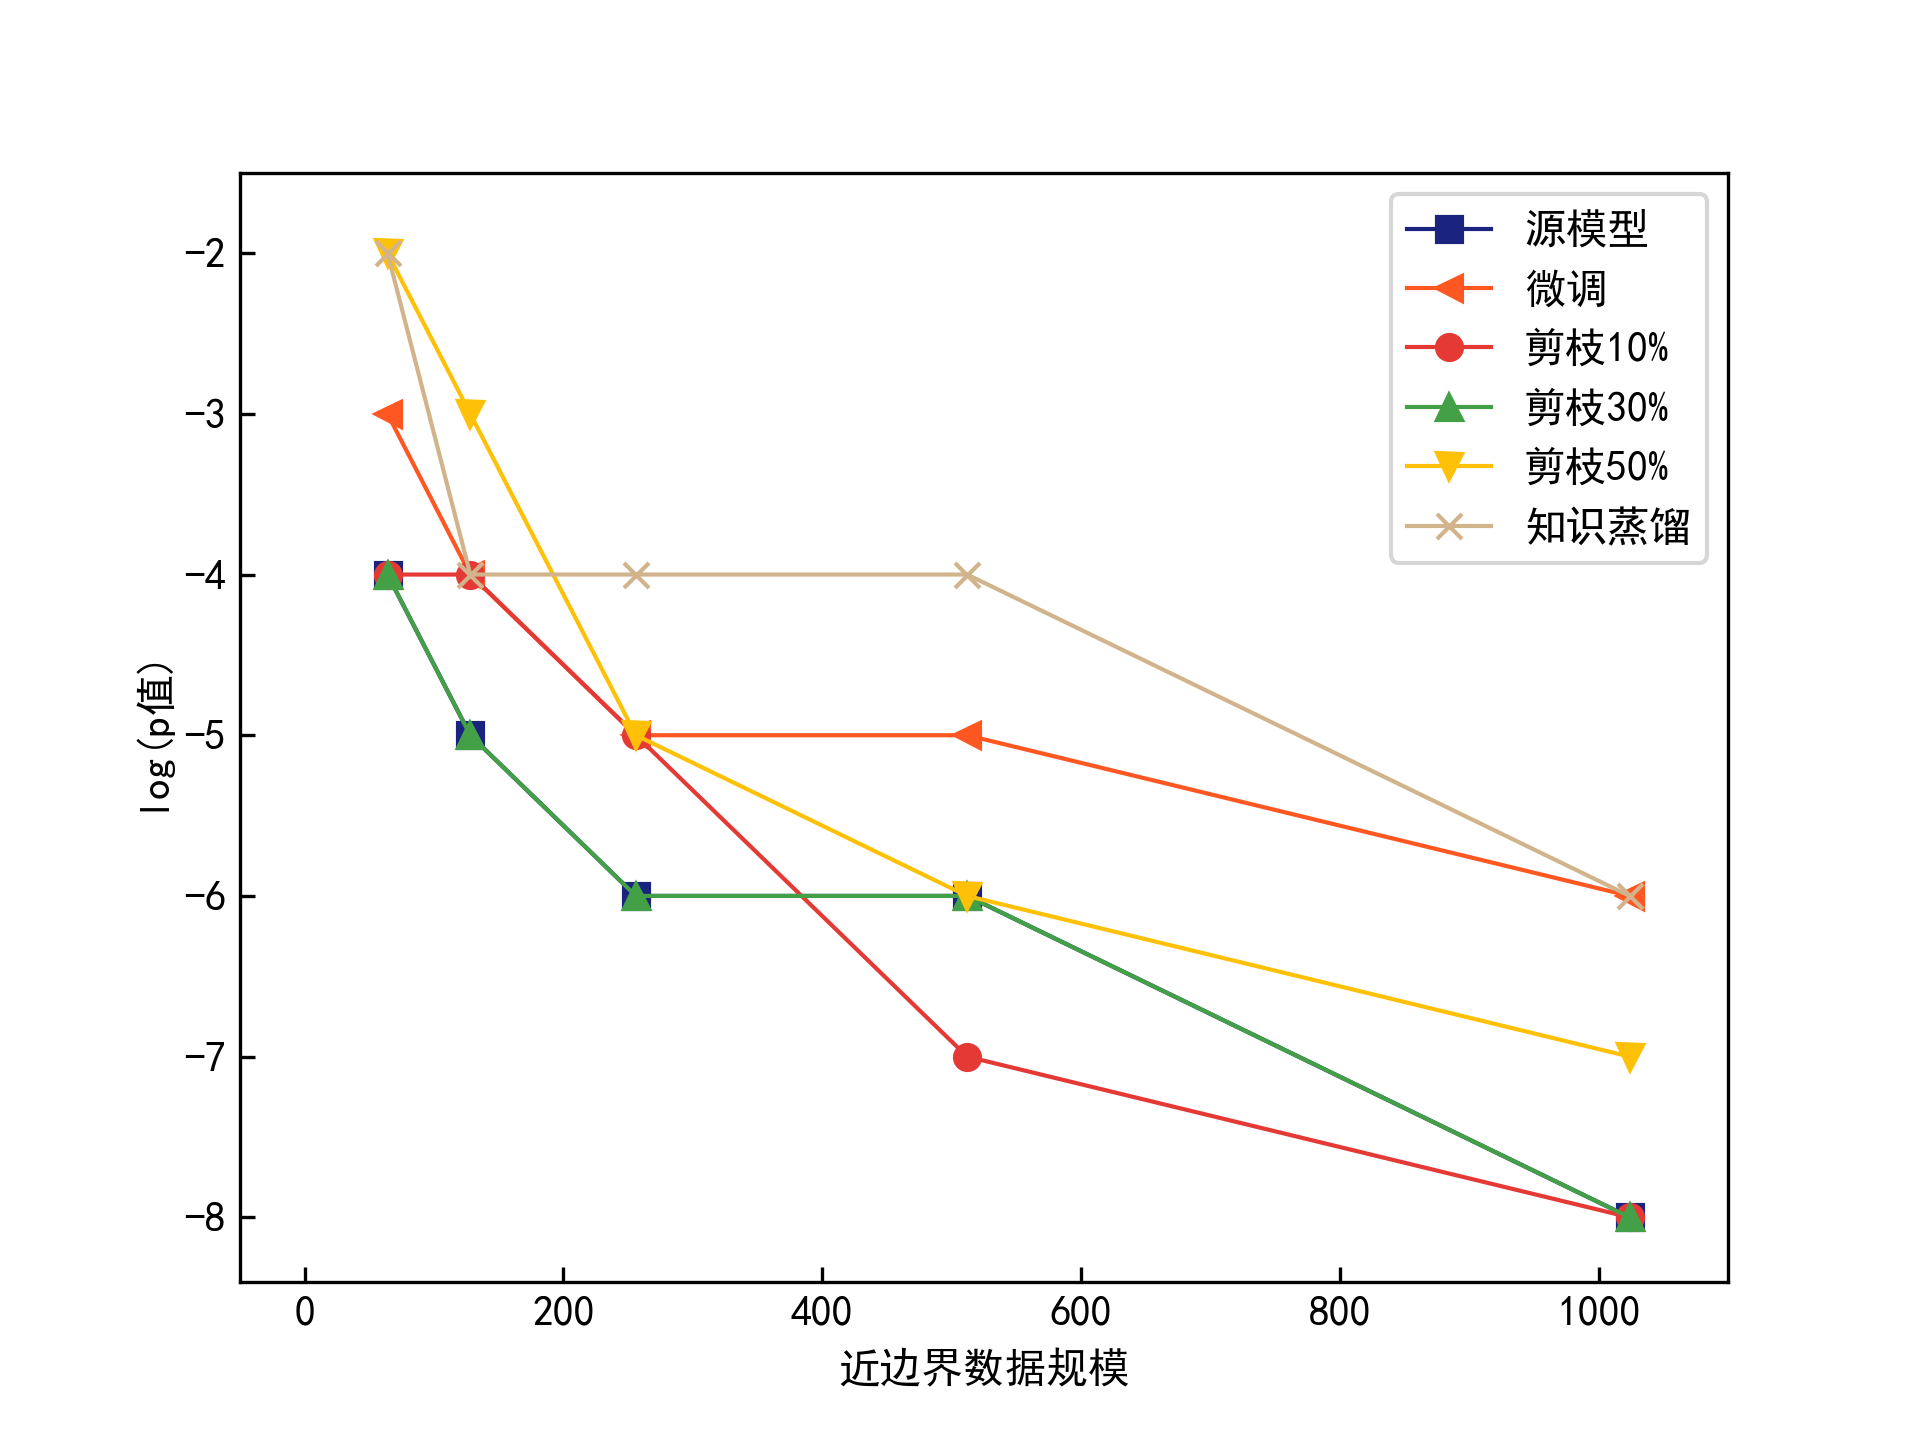
\includegraphics[width=7cm,height=4cm]{CIFAR-10-4-7-p-value.png}
		\centerline{(c)分类边界3}
	\end{minipage}
	\begin{minipage}[htbp]{0.49\linewidth}        %图片占用一行宽度的50%
		\hspace{2mm}
		\centering
		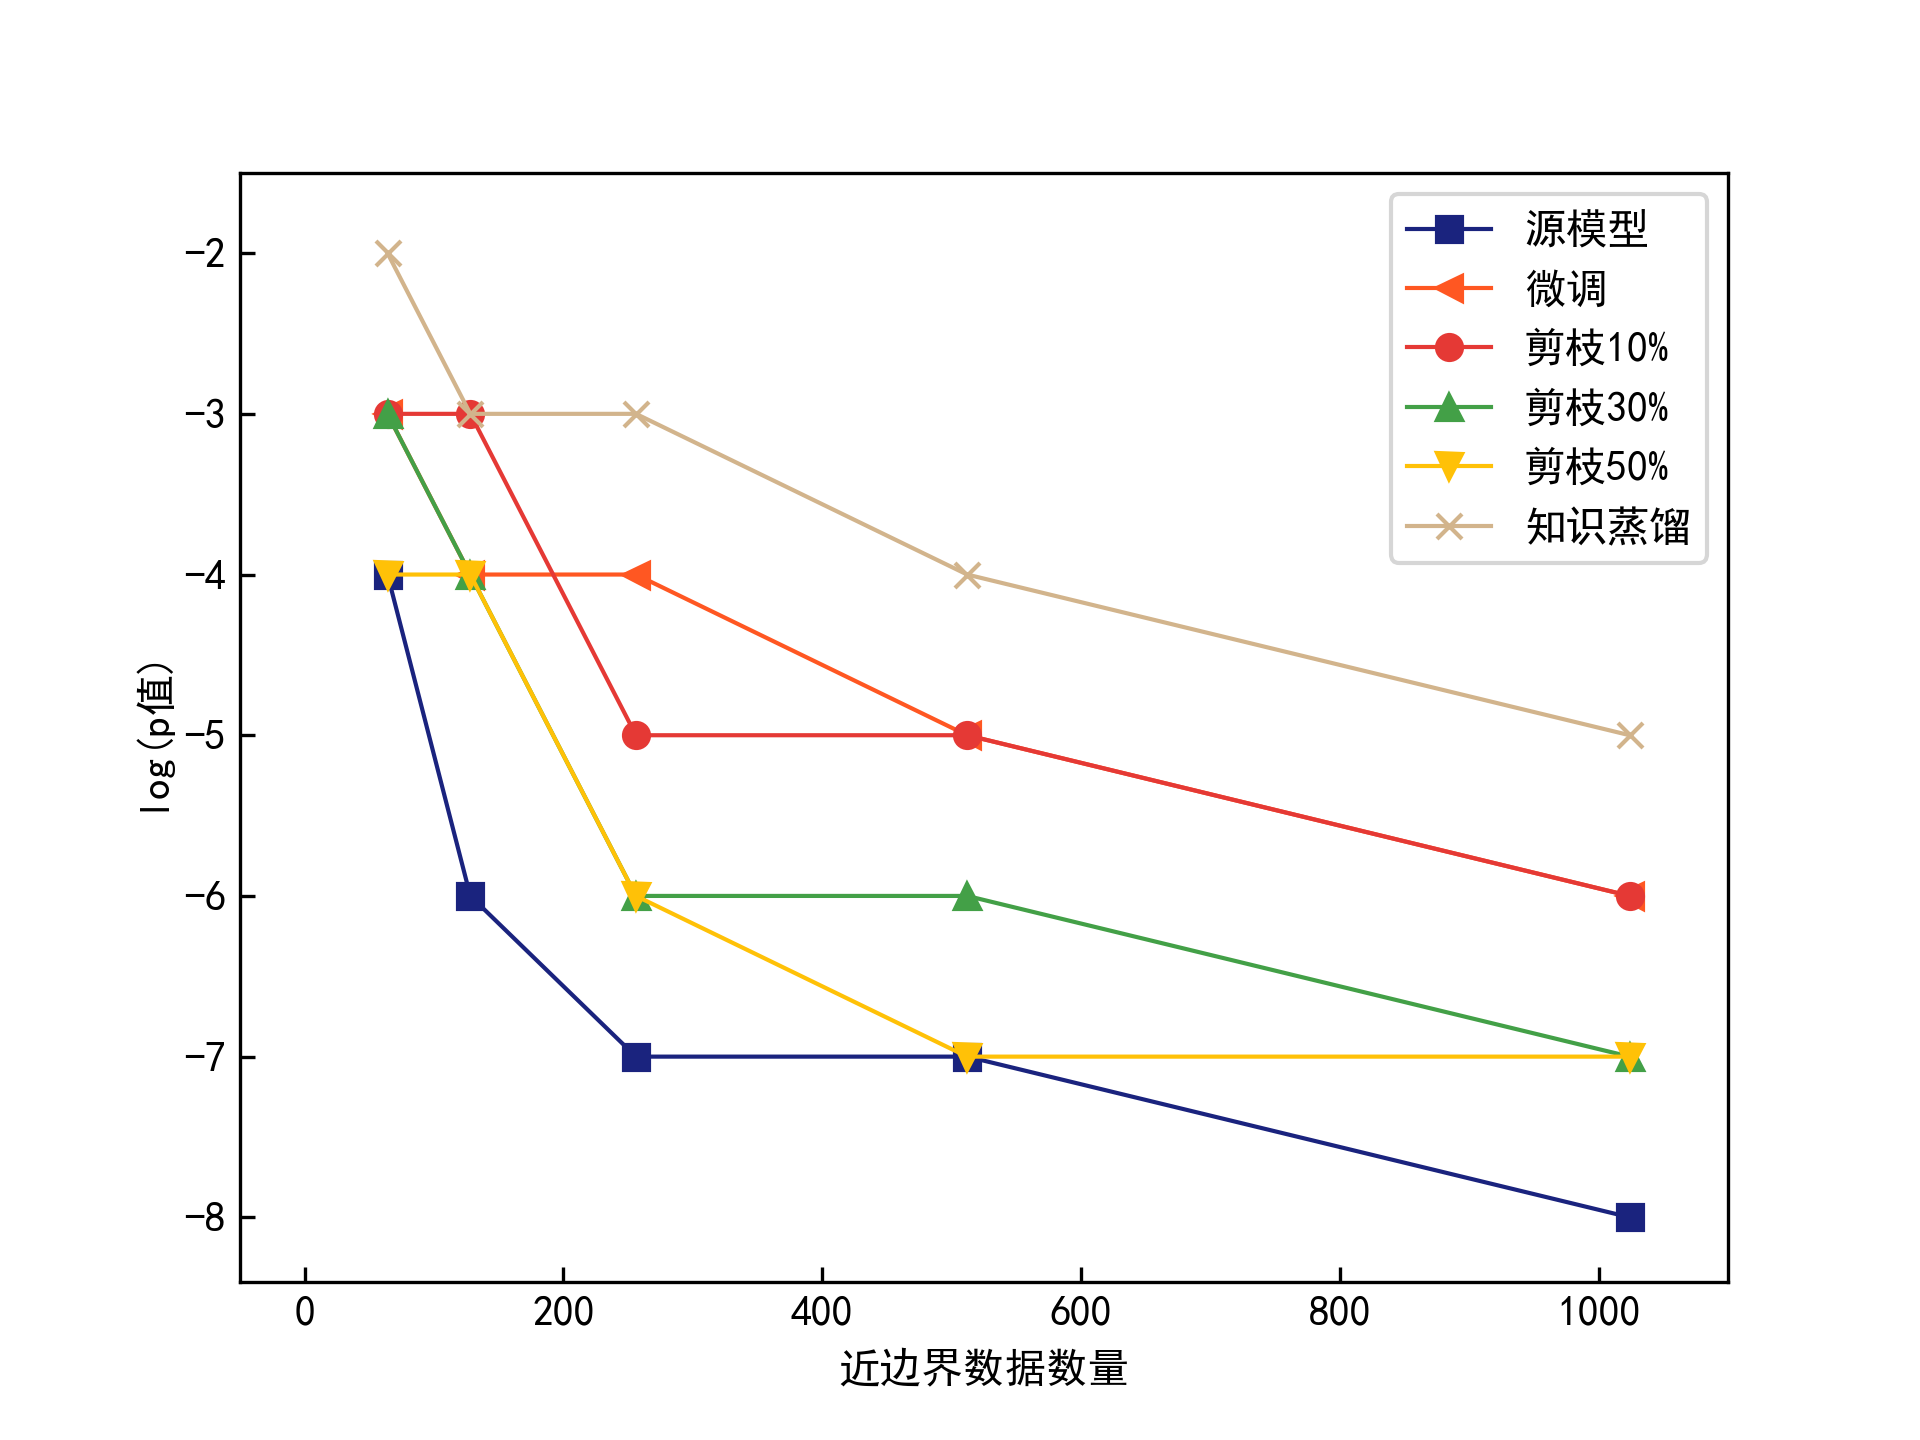
\includegraphics[width=7cm,height=4cm]{CIFAR-10-5-6-p-value.png}
		\centerline{(d)分类边界4}
	\end{minipage}
\setlength{\abovecaptionskip}{7mm} %图片标题与图片距离
\caption{CIFAR-10上推断模型所有权的扩展性}
\label{CIFAR-10上推断模型所有权的扩展性}
\end {figure}
	
\begin{figure}[htbp]%%图,[htbp]是浮动格式
	\centering
	\begin{minipage}[htbp]{0.49\linewidth}        %图片占用一行宽度的50%
		\hspace{2mm}
		\centering
		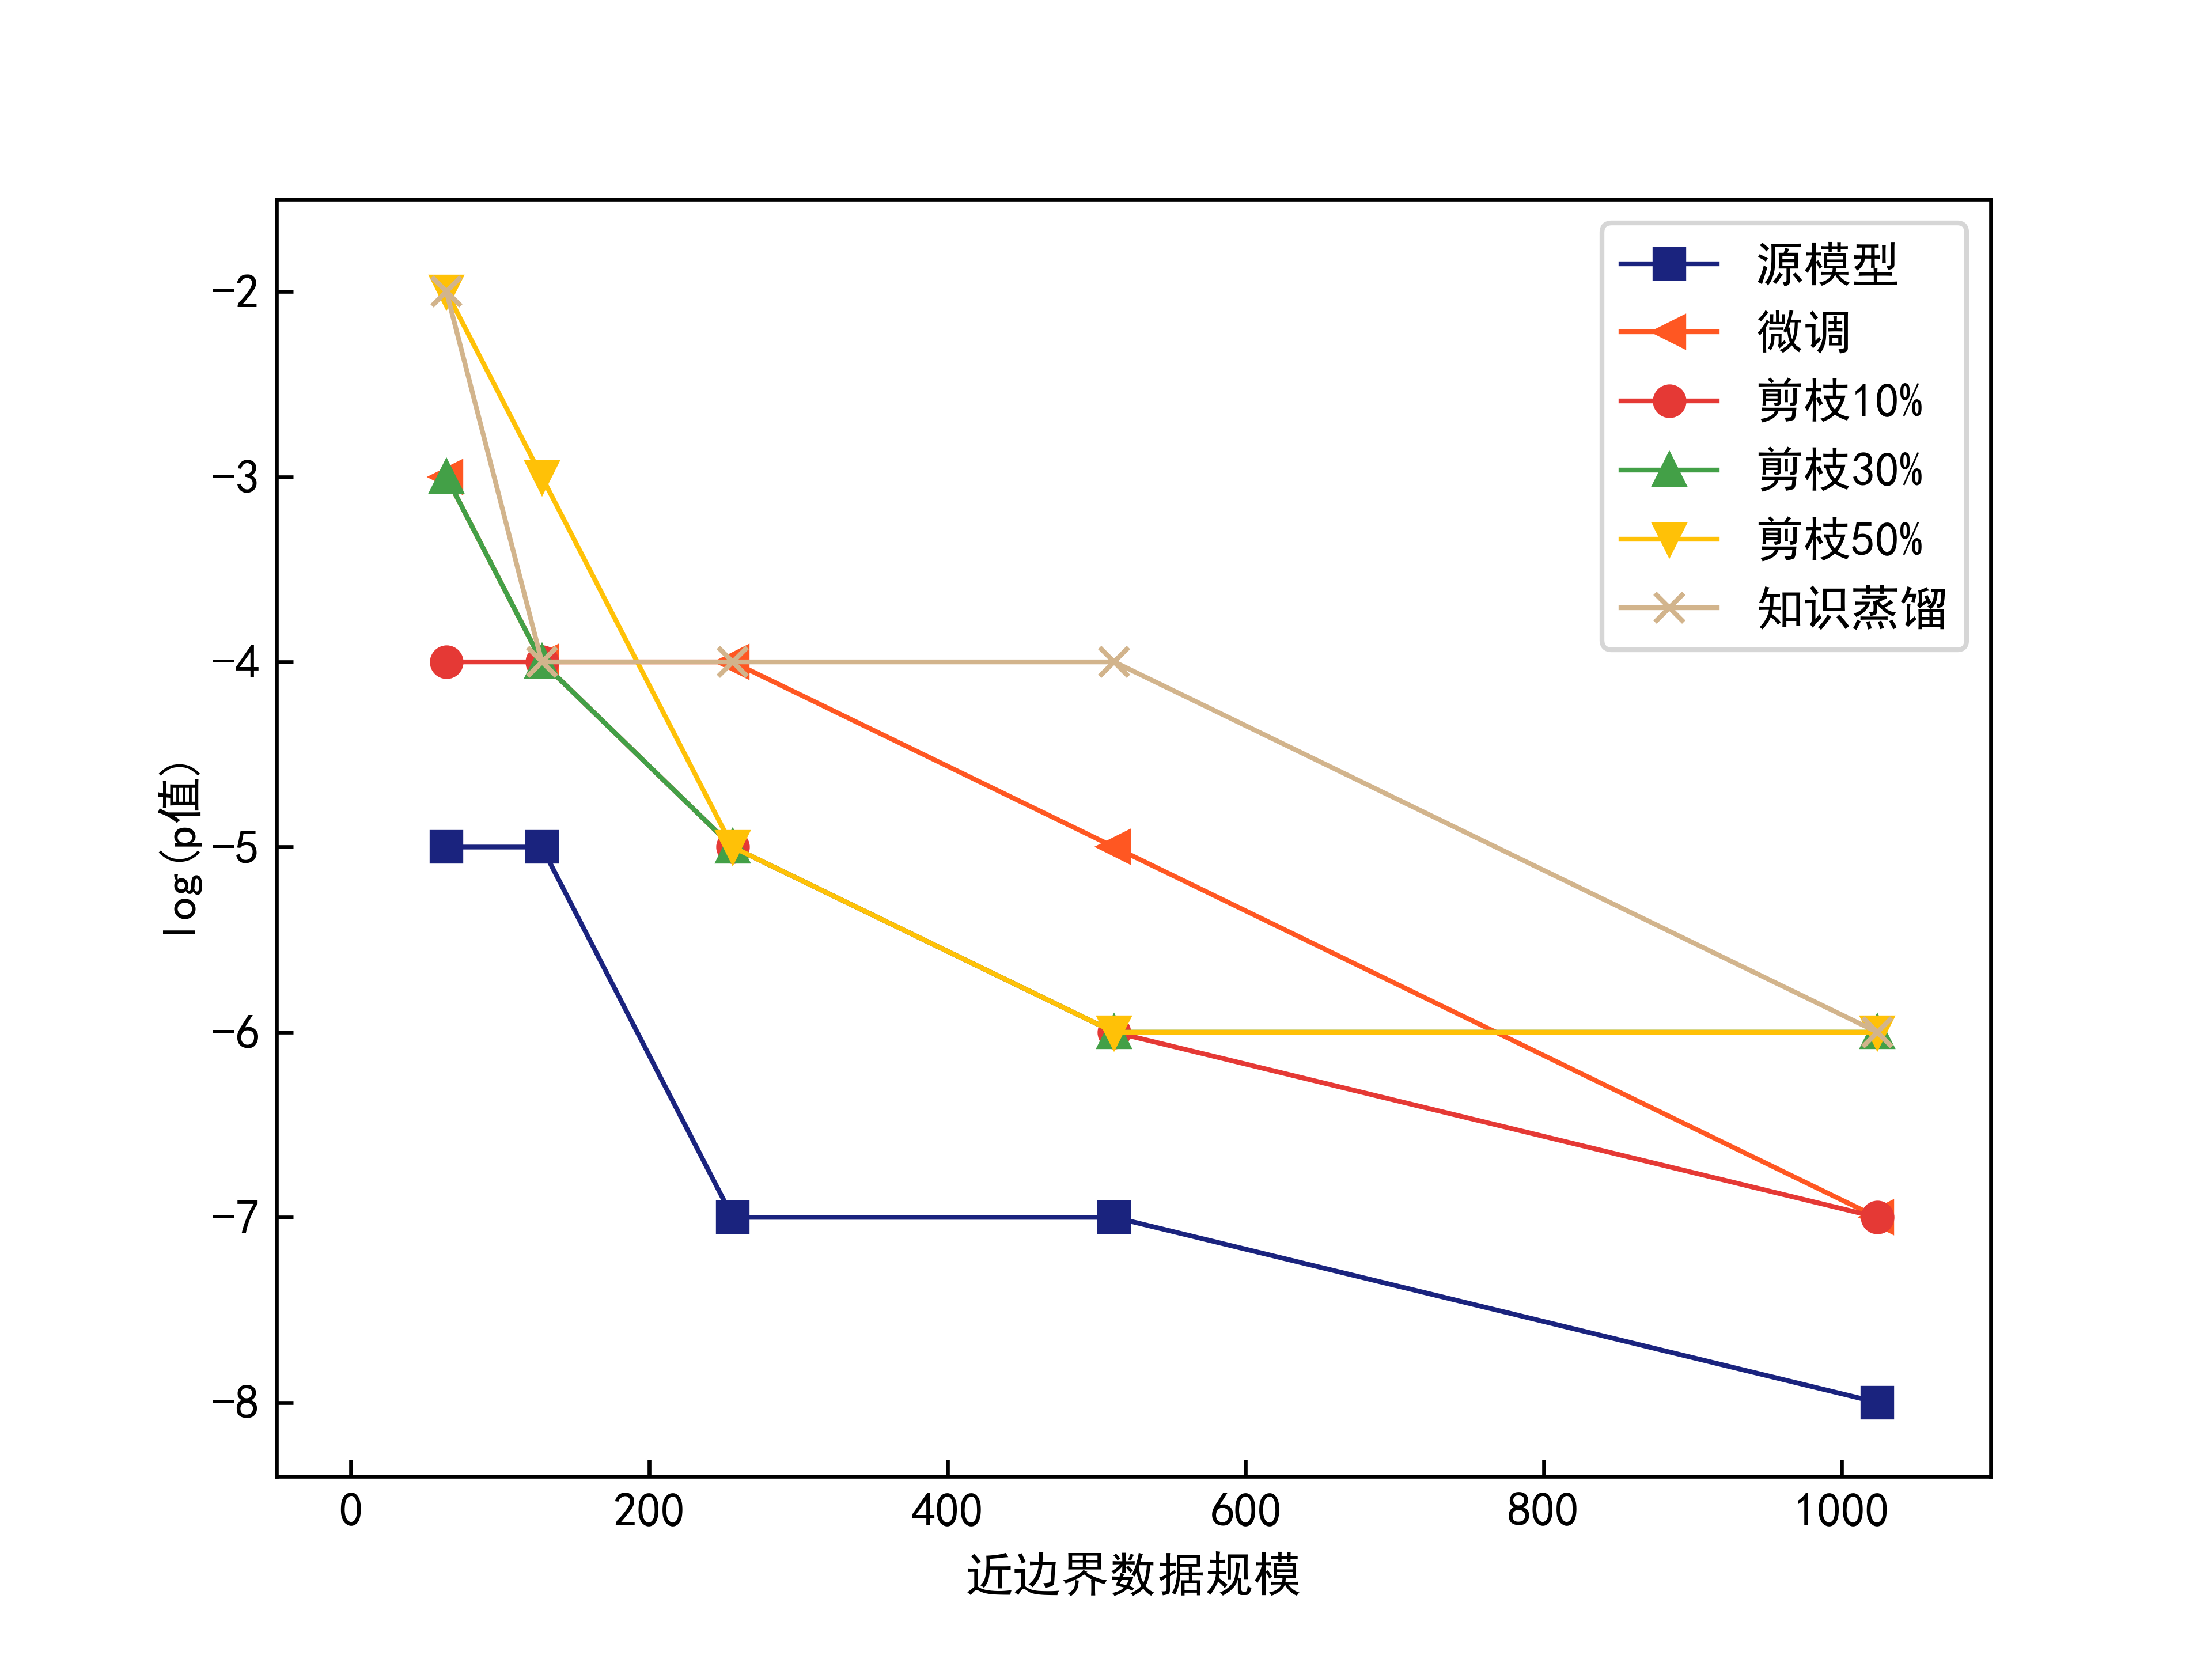
\includegraphics[width=7cm,height=4cm]{Heritage-3-0-p-value.png}
		\centerline{(a)分类边界1}
	\end{minipage}
	\begin{minipage}[htbp]{0.49\linewidth}        %图片占用一行宽度的50%
		\hspace{2mm}
		\centering
		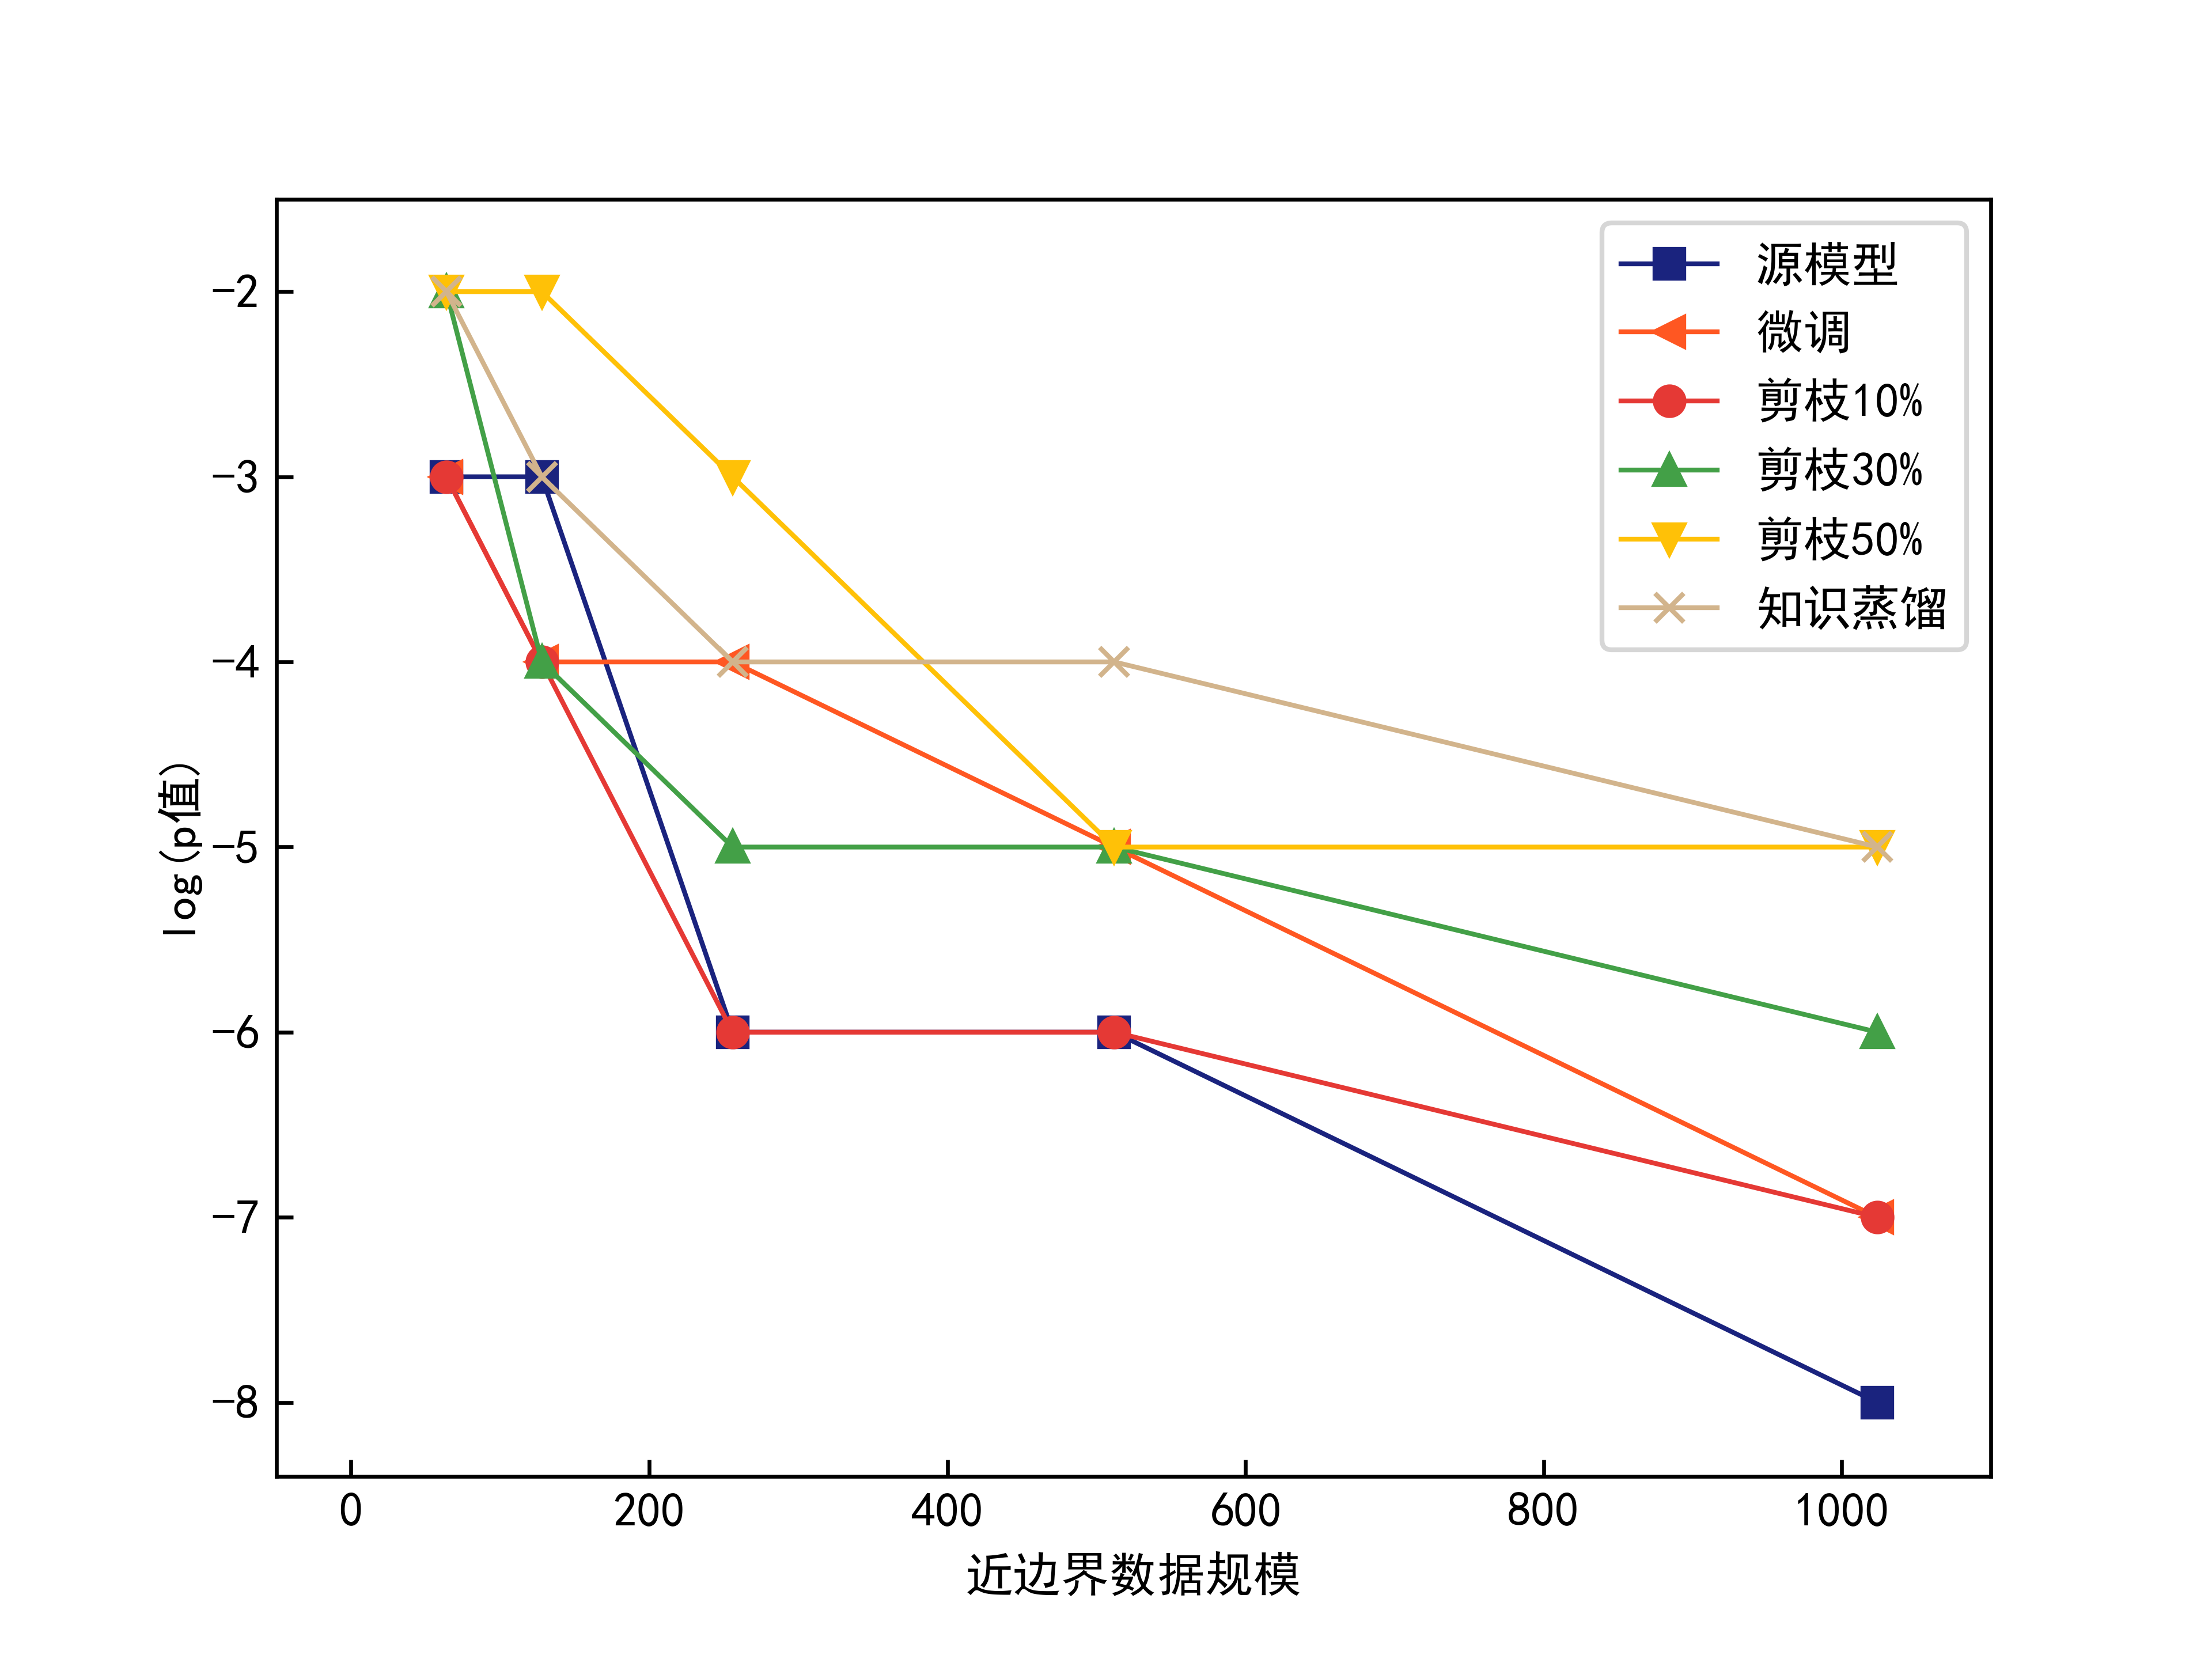
\includegraphics[width=7cm,height=4cm]{Heritage-3-1-p-value.png}
		\centerline{(b)分类边界2}
	\end{minipage}
	\begin{minipage}[htbp]{0.49\linewidth}        %图片占用一行宽度的50%
		\hspace{2mm}
		\centering
		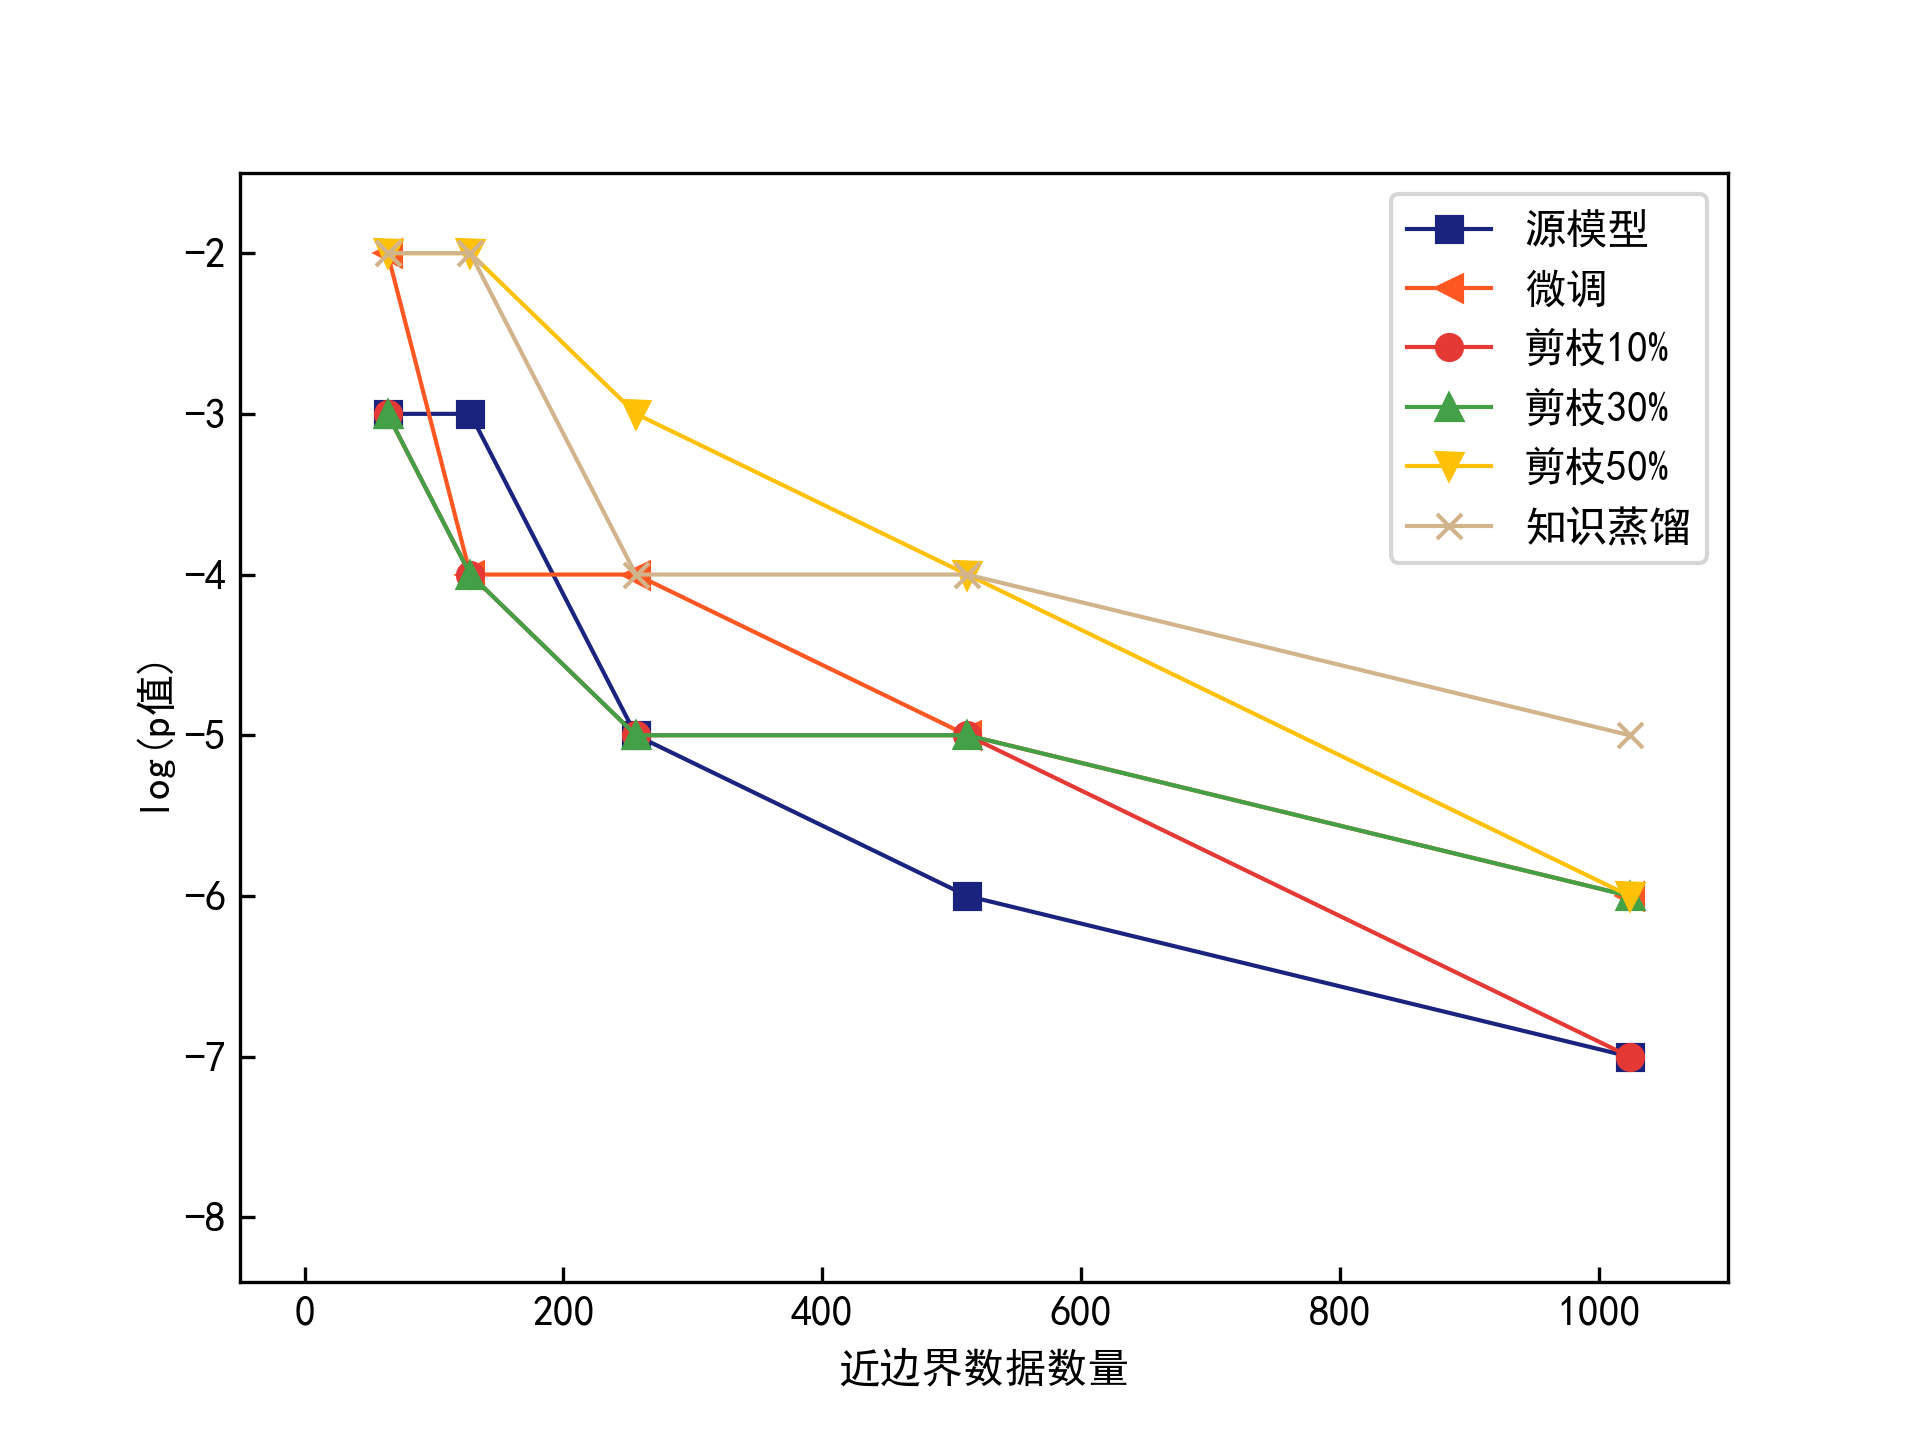
\includegraphics[width=7cm,height=4cm]{Heritage-3-4-p-value.png}
		\centerline{(c)分类边界3}
	\end{minipage}
	\begin{minipage}[htbp]{0.49\linewidth}        %图片占用一行宽度的50%
		\hspace{2mm}
		\centering
		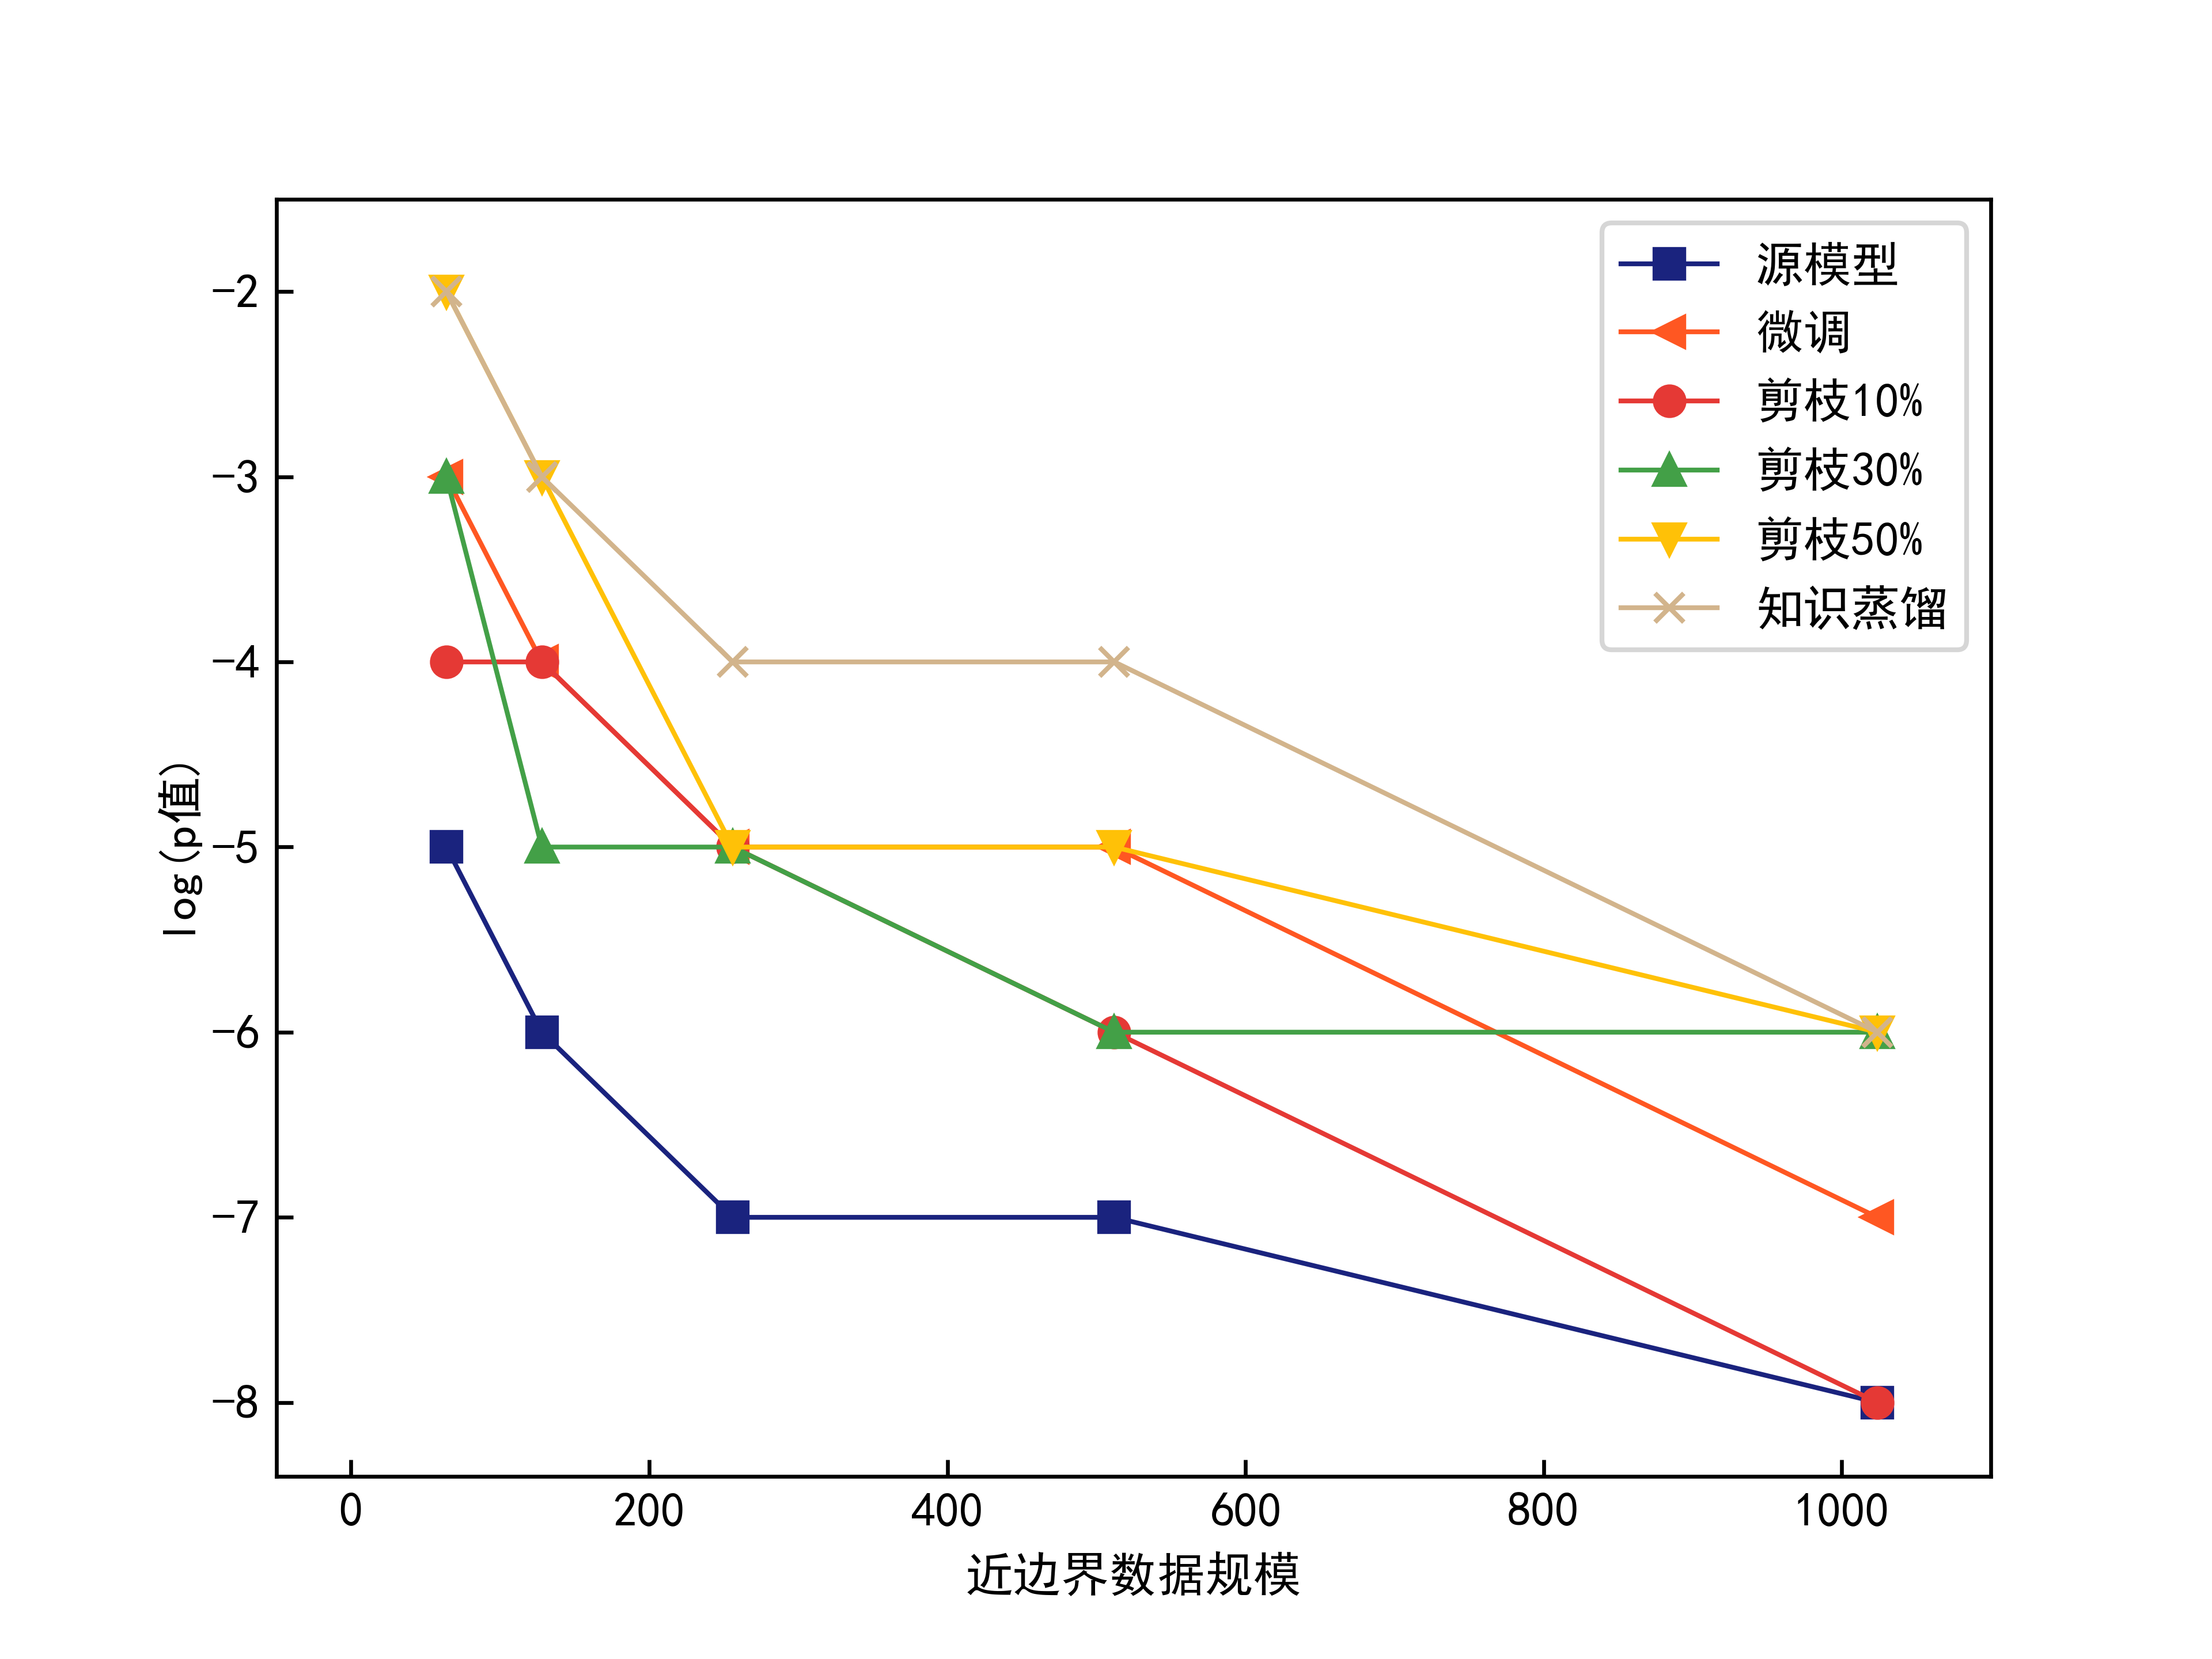
\includegraphics[width=7cm,height=4cm]{Heritage-7-6-p-value.png}
		\centerline{(d)分类边界4}
	\end{minipage}
\setlength{\abovecaptionskip}{7mm} %图片标题与图片距离
\caption{Heritage上推断模型所有权的扩展性}
\label{Heritage上推断模型所有权的扩展性}
\end {figure}
		
\begin{figure}[htbp]%%图,[htbp]是浮动格式
	\centering
	\begin{minipage}[htbp]{0.49\linewidth}        %图片占用一行宽度的50%
		\hspace{2mm}
		\centering
		\includegraphics[width=7cm,height=4cm]{Intel\_image-3-1-p-value.png}
		\centerline{(a)分类边界1}
	\end{minipage}
	\begin{minipage}[htbp]{0.49\linewidth}        %图片占用一行宽度的50%
		\hspace{2mm}
		\centering
		\includegraphics[width=7cm,height=4cm]{Intel\_image-3-4-p-value.png}
		\centerline{(b)分类边界2}
	\end{minipage}
	\begin{minipage}[htbp]{0.49\linewidth}        %图片占用一行宽度的50%
		\hspace{2mm}
		\centering
		\includegraphics[width=7cm,height=4cm]{Intel\_image-3-5-p-value.png}
		\centerline{(c)分类边界3}
	\end{minipage}
	\begin{minipage}[htbp]{0.49\linewidth}        %图片占用一行宽度的50%
		\hspace{2mm}
		\centering
		\includegraphics[width=7cm,height=4cm]{Intel\_image-5-0-p-value.png}
		\centerline{(d)分类边界4}
	\end{minipage}
\setlength{\abovecaptionskip}{7mm} %图片标题与图片距离
\caption{Intel\_image上推断模型所有权的扩展性}
\label{Intel-image上推断模型所有权的扩展性}
\end {figure}

\section{本章小结}

本章从多个方面测试了我们方法的各个指标,有效的证明了我们提出的方法的有效性。


